\documentclass[12pt]{article}

%AMS-TeX packages
\usepackage{amssymb,amsmath} 
\usepackage{geometry, graphicx}
\usepackage{caption}
\usepackage{physics}

\usepackage[normalem]{ulem}
\useunder{\uline}{\ul}{}
\usepackage{longtable}

% setup the margins
\geometry{margin=1.0in, headheight=15pt}

\graphicspath{ {../lab04/images} }    


\begin{document}

\title{PHSX 444: Lab 04; Paul Trap for Charged Particles}
\author{William Jardee}
\maketitle


\section{Introduction}
%% Introduction section. Here I introduce the physics of the experiment and give some slight motivation for the experiment. I personally think that putting the physics of the apparatus here is better. 

Particle traps are a fundamental cornerstone to many lab settings, from precise measurements to measure specific characteristics such as excitation levels. While many use fancy setups that rely on advanced procedures and exact execution, there are some pit-stops along the way that students can use to get a hands on understanding of the physics of particle traps, without as much difficulty. One of these ``pitstops" is the Paul Trap. The Paul Trap is a type of electrodynamics ion trap (EIT). By using an oscillating electric field, such as from an AC current, the position of a charged particle will find an equilibrium point in the center of the trap. Figure \ref{fig:paul_trap_diagram} shows the general setup, however this is a very unstable design. The edges of the bars that make the top of the trap can be curved to create a concave basis that holds the particle in with gravity. A stable region can also be accomplished with a quadruple setup. The one that will be implemented here will instead be a circular structure, where the two plates in Figure \ref{fig:paul_trap_diagram} can be though of as a toroid coming in and out of the paper. This toroid will create a pulsing field in and out of the center or the shape. Some fun calculations give the expected force on the particle:
\begin{equation*}
z \approx -\frac{q E}{m \omega^2}\sin(\omega t)
\end{equation*}
\begin{equation*}
\ev{F_z(z,t)} \approx -\frac{1}{2} \frac{qE_0 E^\prime}{m \omega^2}
\end{equation*}
and so on. However, those calculations won't be used here. Instead, the focus will instead be on the Boltzmann distribution of the thermal energy and how it relates to the mass. 

\begin{figure}[ht]
\centering
    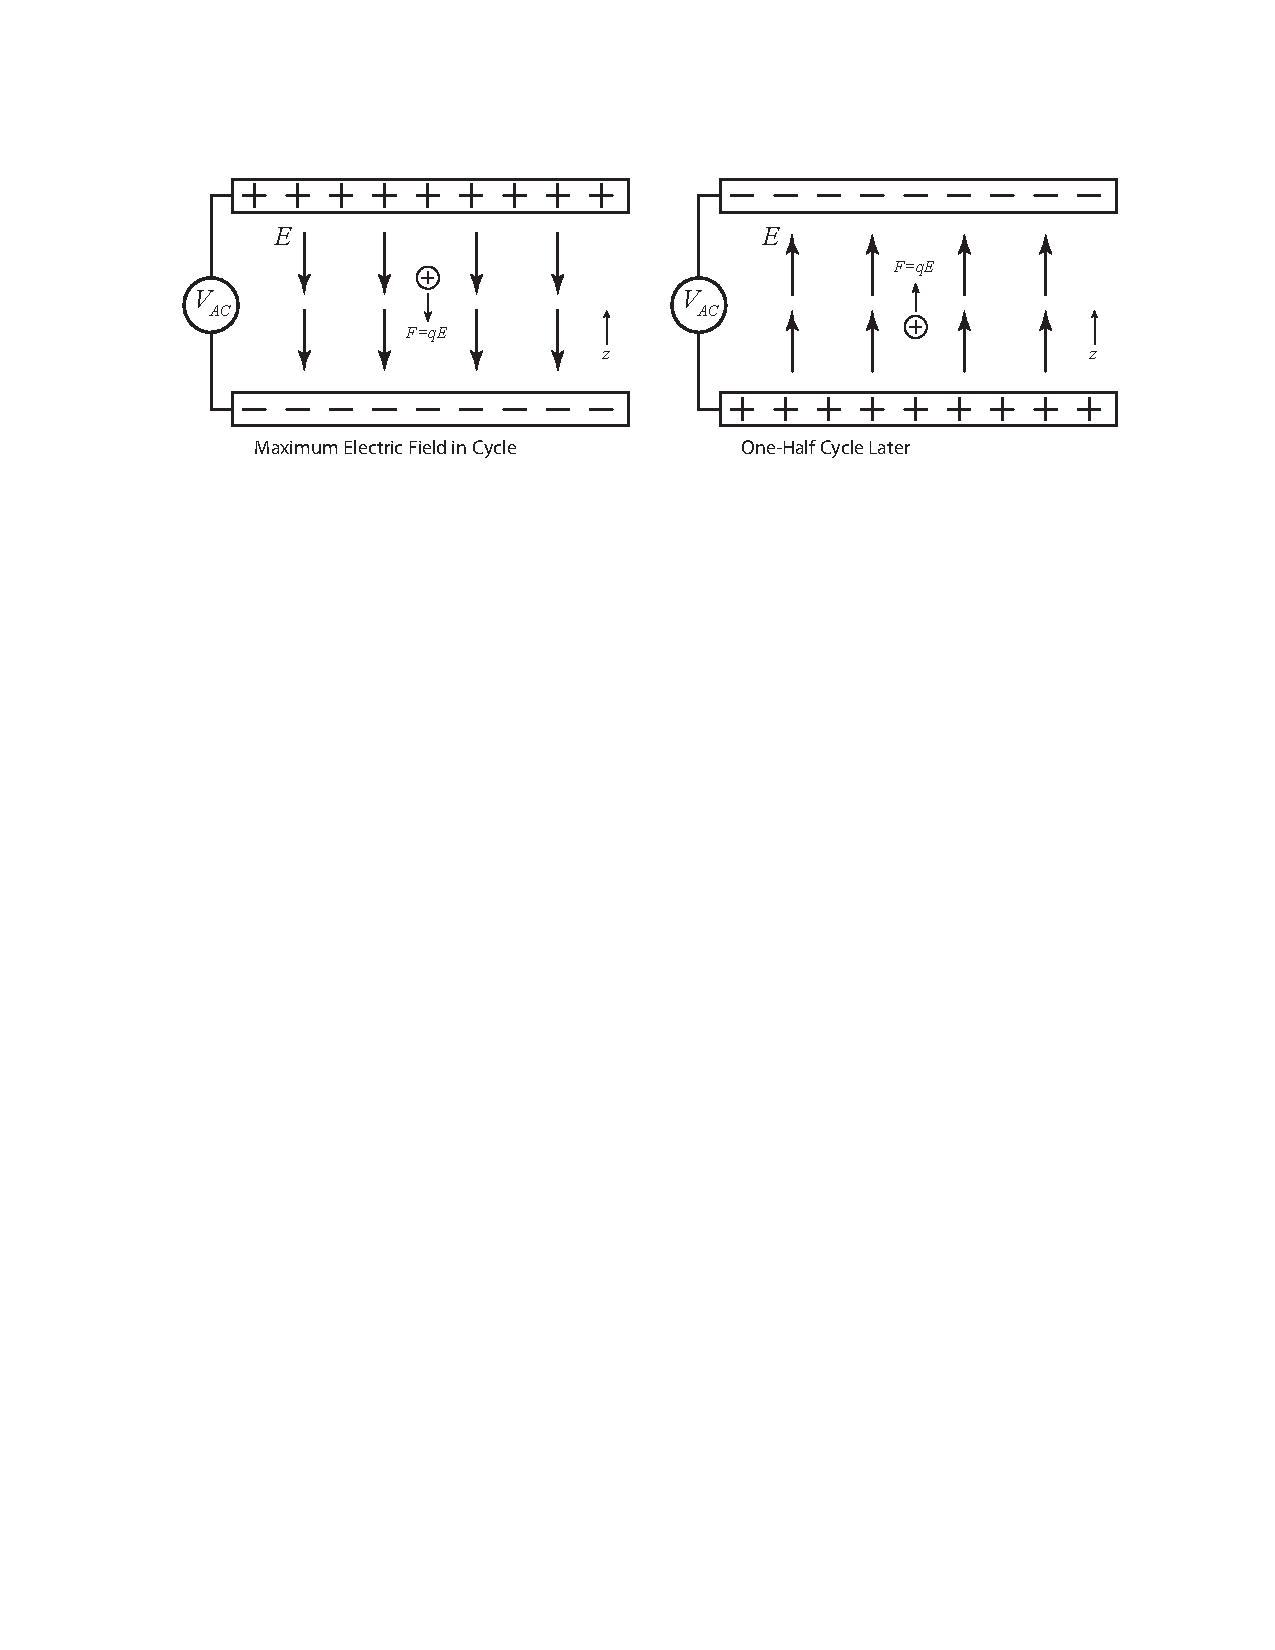
\includegraphics[width=\textwidth]{paul_trap_diagram.pdf}
	\caption{}
    \label{fig:paul_trap_diagram}
\end{figure}

For a general particle in a simple harmonic oscillator, the probability that a particle is found at a certain energy with $v_i$ and $x_i$ is:
\begin{equation*}
P(x_i, v_i) = \textbf{exp}\Big(-\frac{\frac{1}{2}mv_i^2 + \frac{1}{2}m\omega_i^2x_i^2}{k_B T}\Big)
\label{eq:gen_prob}
\end{equation*}
Marginalizing out the positional argument by integrating over $x$ provides:
\begin{equation*}
P(v_i) \propto \textbf{exp} \Big( -\frac{mv_i^2}{2 k_B T}\Big)
\label{eq:marg_prob}
\end{equation*}
And taking the natural log of this, introducing a normalization constant $\ln(A) = A^\prime$:
\begin{equation}
\ln[P(v_i)] = -\Big(\frac{m}{2k_B T}\Big) v_i^2 + A^\prime
\label{eq:marg_prob2}
\end{equation}
Where $m$ is the mass or the particle, $\omega$ is the oscillation frequency, $k_B$ is the Boltzmann constant, and $T$ is the temperature. 

%-----------------------------------------------------------------------

\section{Experimental Methods}
%% Go into depth about the setup of the components, shit used, and any specs that are useful to know.
\begin{figure}[ht]
\centering
    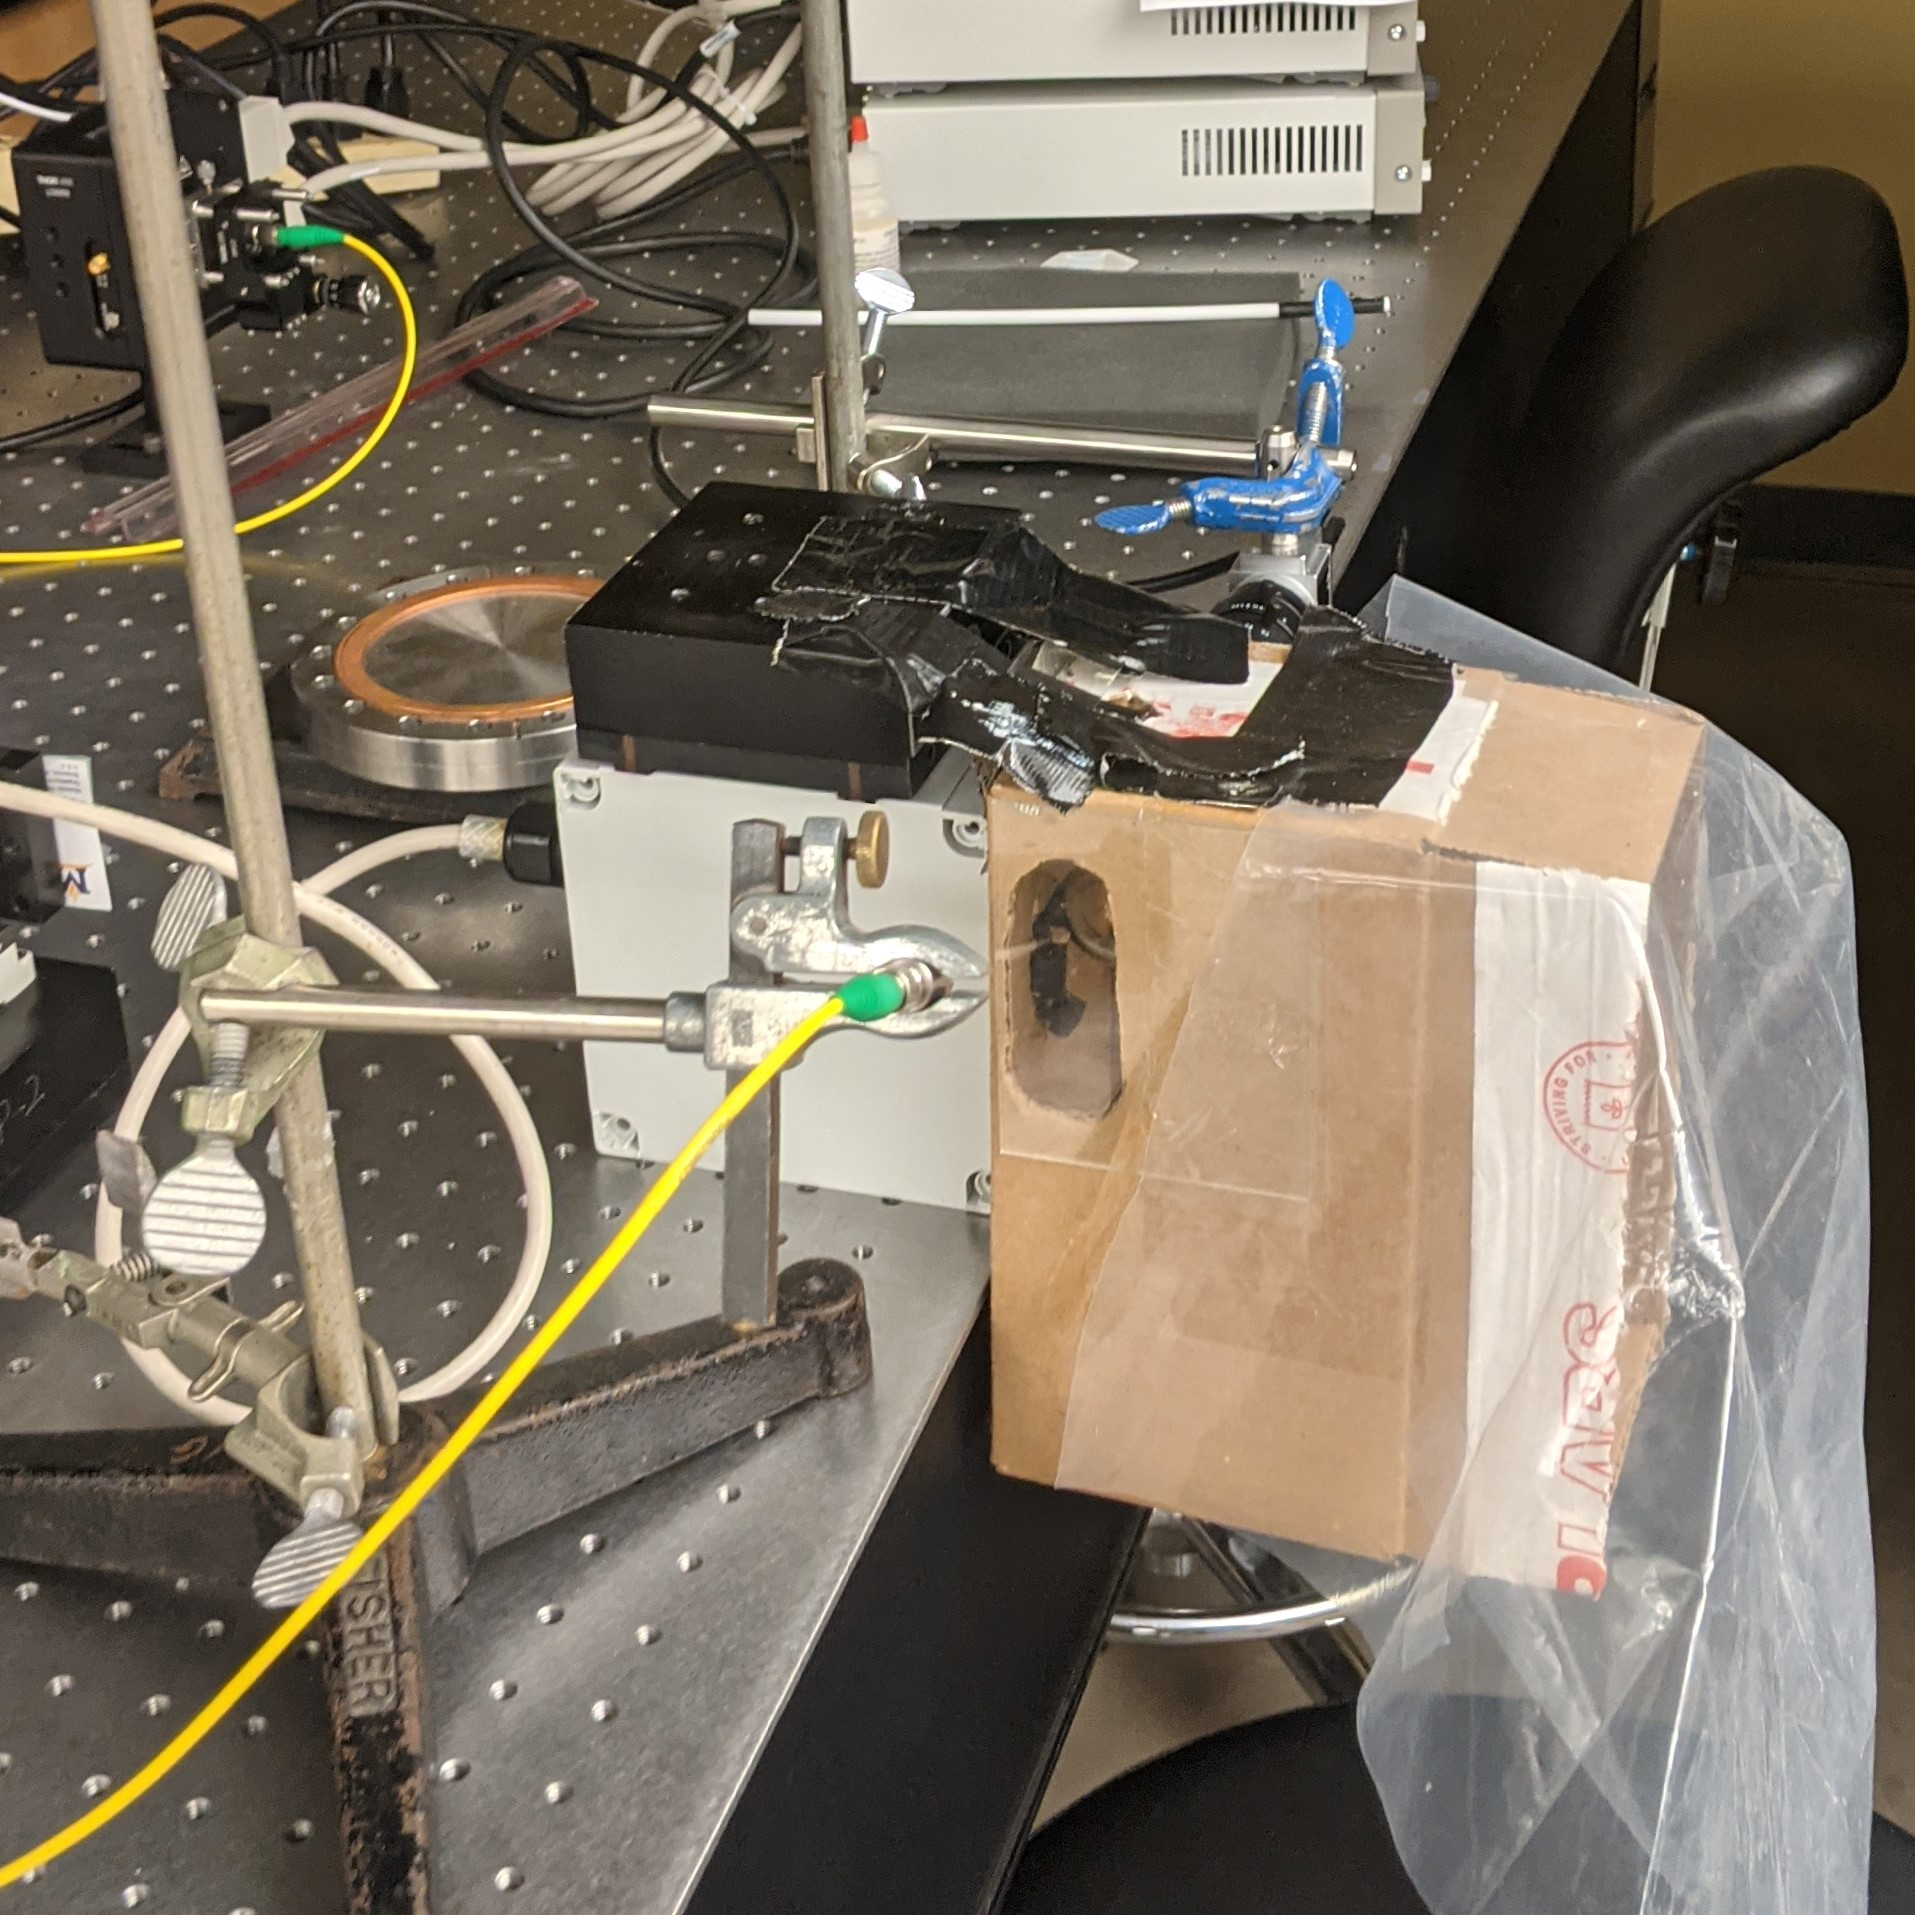
\includegraphics[width=0.5\textwidth]{paul_trap.jpg}
	\caption{A diagram of a simple paul trap via \cite{pauly}}
    \label{fig:paul_trap}
\end{figure}

The Paul Trap was constructed using a variable voltage regulator to provide an AC source at 60 Hz with a range of 0-135 V. This AC source was connected up to an I-ring screw. To protect the trap from external air currents, a high-tech cardboard box surrounded the trap, with two oval slits in the side, running parallel to the ground and covered with thick, clear plastic to create a sort of viewing window. (See figure \ref{fig:paul_trap}). To continue minimizing the impact of air currents, the door was closed and a drape was pulled closed behind the trap. Even with these procautions, it will seen that air currents seemed to contribute a large to the collected data, to the point of making an analysis impossible. 

The particles used in the trap were Lycopodium, commonly called Dragon's Breathe because of it's use by magic hobbyists. Using a plastic dowel that was rubbed on some foam to pick up a slight electric charge, lycompods were picked up, and simutaneously charged, and dropped into the apparatus from a small hole in the top of the box. This hole had a slide cover to allow the box to be resealed when the hole was not needed. As the particles floated through the trapping region, a collection of them would get trapped. For most of the analysis, only one particle was wanted, so a dust blower was used to introduce a puff of air that would knock unwanted particles away. This proved surprisingly effective. 

The trap was observed using a camera fitted with a $0.3\times - 1\times$, $1:45$ zoom lens. Since the zoom changes the pixel scale, each time the focus was changed a new set of calibration pictures had to be taken. By using a monochromatic laser and taking a very small window of focus, the framerate of the camera was able to toggled, up towards the rate of 200 fps, for a $200 \times 200$ window. The rate was able to go up towards 300 fps, but that required the window size to be on an order that removed the particle from some of the frames. 


\subsection{Calibration}
%% Talk about the importance of the calibration slide
\begin{figure}[ht]
\centering
    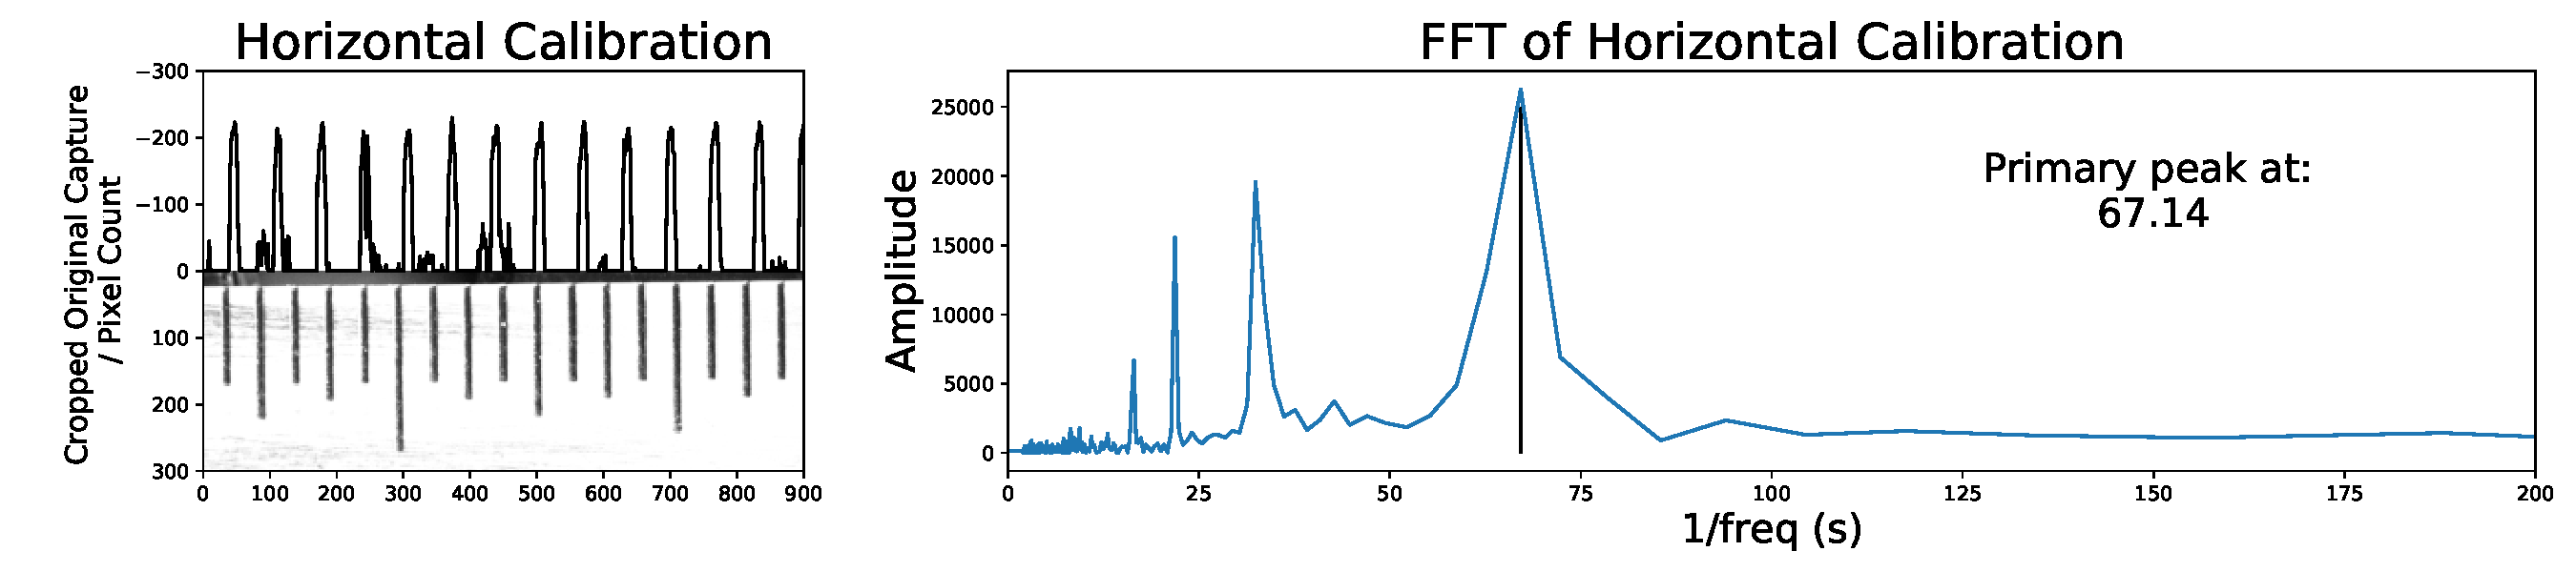
\includegraphics[width=\textwidth]{hori_cali.pdf}
    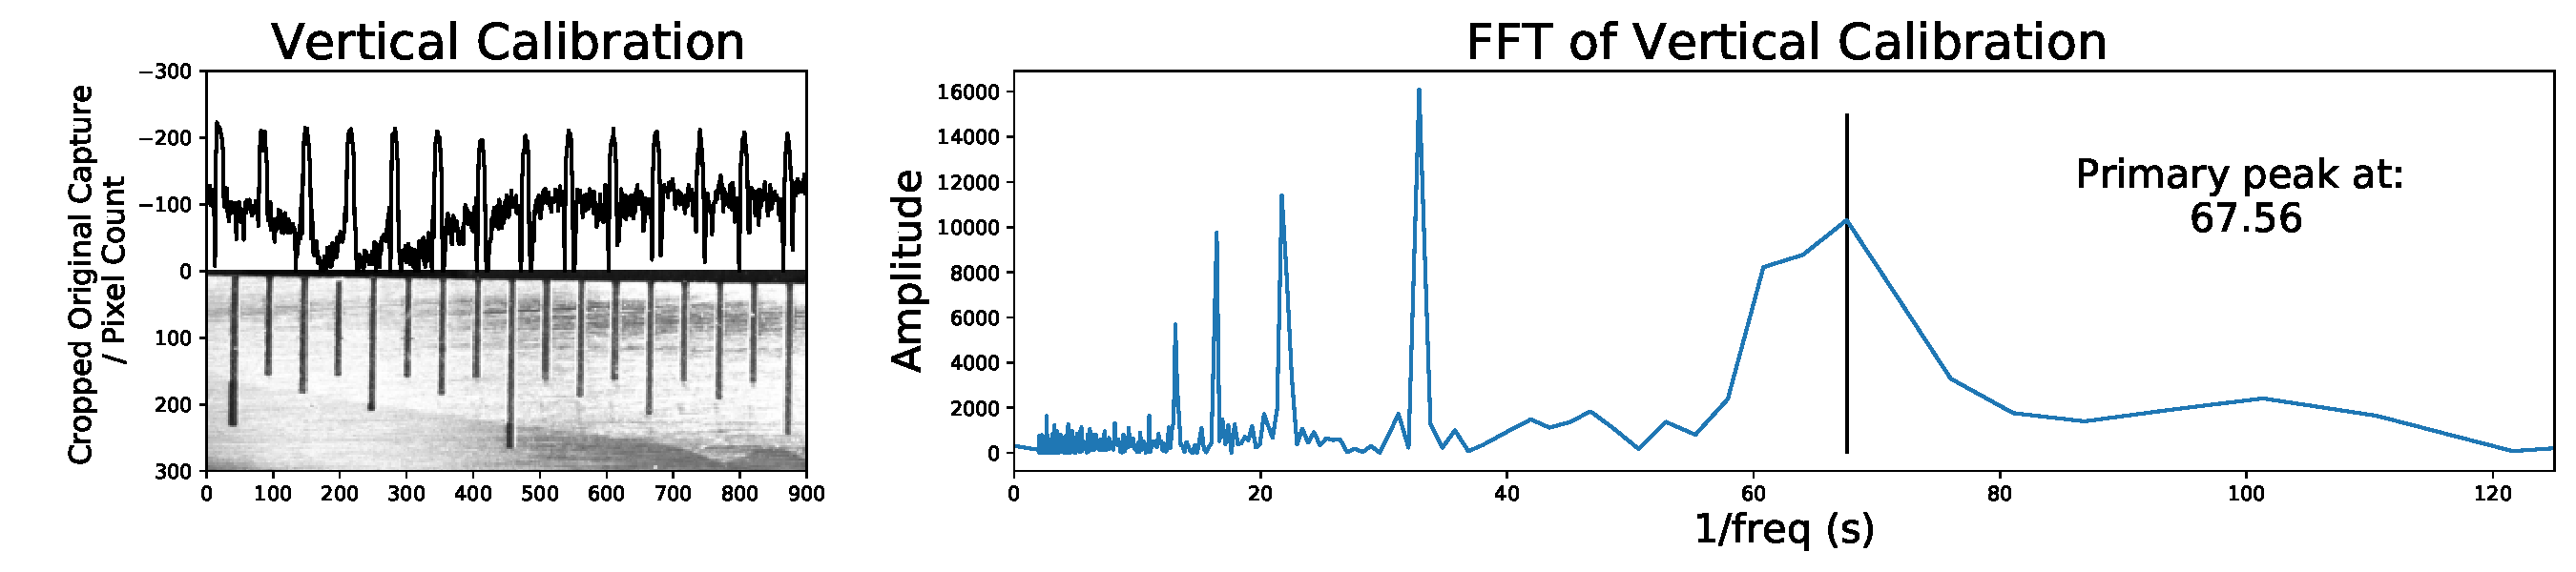
\includegraphics[width=\textwidth]{vert_cali.pdf}
	\caption{The calibration of the camera zoom used. It can be seen that the interesting peak is about 67 pix/mm in both directions.}
    \label{fig:calibration}
\end{figure}
To calibrate the camera, two images were taken of a standard desktop ruler; one in the horizontal configuration and one in the vertical. These two images were then sliced along a line to get the magnitude count down the side of the ruler. This oscillatory behavior was then analyzed in the Fourier domain to get the primary width between peaks. This served to give the pixel to millimeter ratio. As can be seen in the Fourier images of Figure \ref{fig:calibration}, the resolution of the FFT was not overly impressive, but there is a clear primary peak around 66 (pixels per a mm) in the horizontal and 67 (pixels per a mm) in the vertical.



\subsection{Data Collection Errors}
%% The method that we used to collect data and the critical failures that meant that we could not use our data
The setup show is obviously a thrown together system that has been proven to work in the ideal circumstances. The shield blocks a moderate amount of air currents, but currents that are able to enter from the bottom of the box tend to be a big issue. In the data collection, the data points to the fact that the bottom of the plastic sheet was not pulled tight against the box, and so the data was extremely messy (as can be see in Figure \ref{fig:flawed_pos}. It also would seem that what the software collected and what was told to be collected seemed to disagree. While screenshots of the capture software communicate that the frame rate of was 200 fps, the characteristics seemed very close to those of the 60 fps (Figure \ref{fig:flawed_pos}). This is both for the analyzed data and the raw footage. It needs to be investigated whether the frame rate taken corresponds to the capture software input or the settings imported from the another software.

So, all the data that was collected by our group was unusable. Reaching out to another group who had neither of these errors, supplementary data that held very good characteristics of both micro-motion and secular motion. The data gathered was collected at 60 Hz, 61 Hz, and 198 Hz. The 60 Hz and 198 Hz both had captures of a transient response from bumping the table with a fist. The collection time for the 60 Hz, 61 Hz and both transient data were 3000 frames. The 198 Hz had much more data, with 15000 frames. Nearly all the data that will be shown will be from these 5 data sets; with the exception of Figures \ref{fig:flawed_pos}, and \ref{fig:flawed_vel}, which are provided to show how unreliable that data is. 

%-----------------------------------------------------------------------

\section{Results and Analysis}
%% Bring up the premise that only group 2 data will be provided in depth
The data analysis proved to be a great learning experience. Communicating with out groups, it turned out that there were a couple crucial errors that were made. This was a great learning experience about analyzing data in between sessions so there would be time to fix any errors before the allotted time is over. 

\subsection{Flawed Data Analysis}
%% The full process will be given in the next subsection, just see that it don't work well
\begin{figure}[!ht]
\centering
    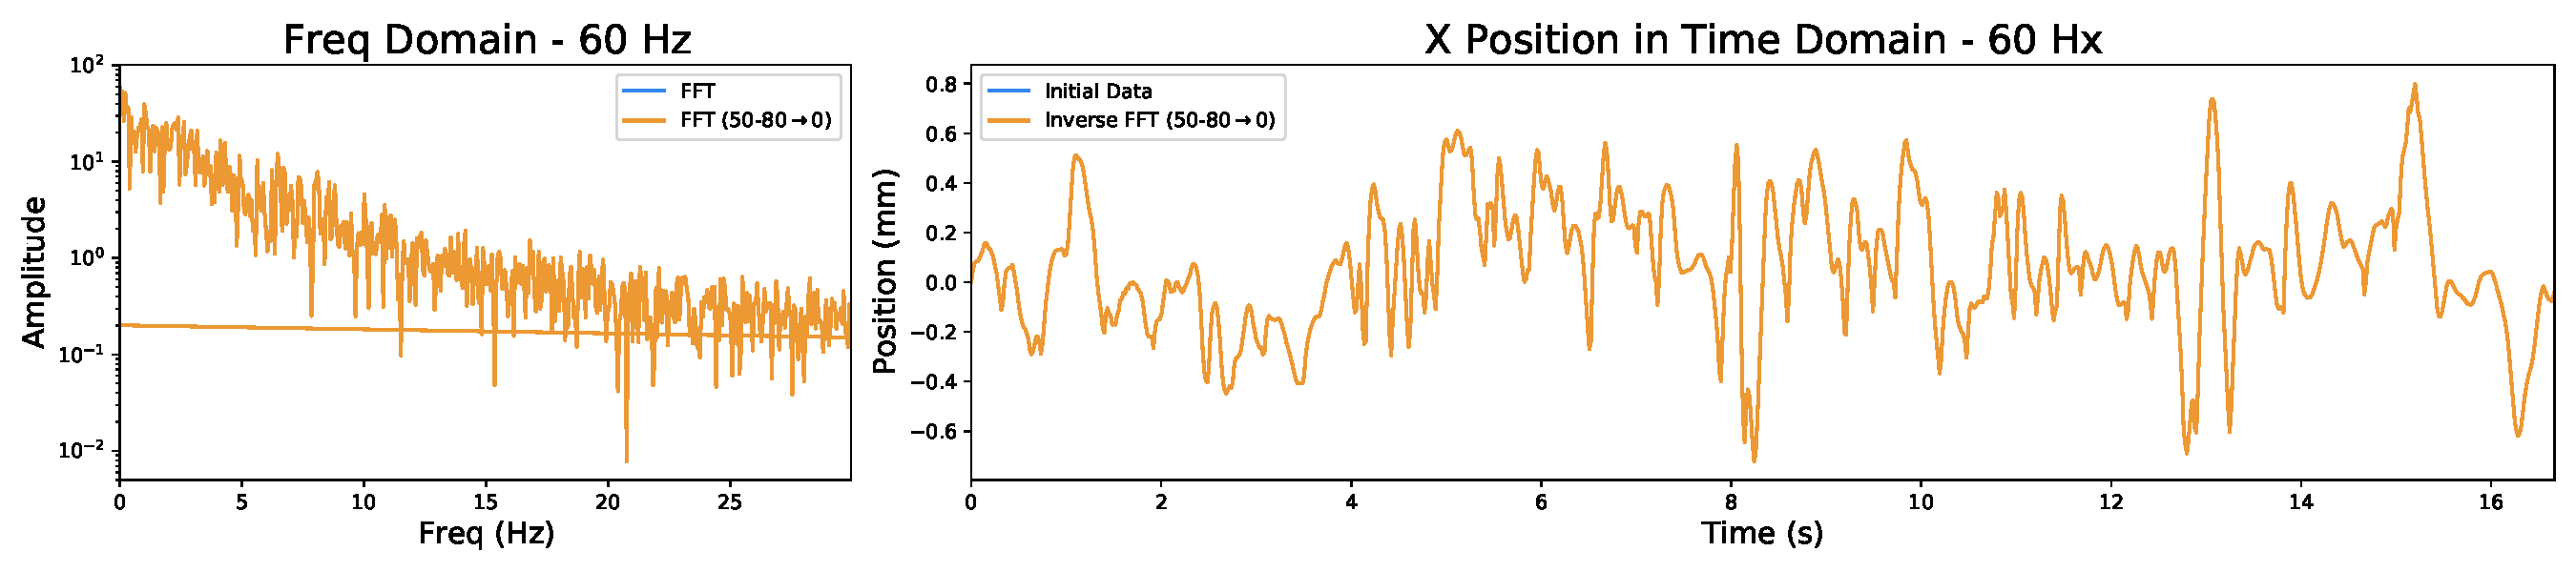
\includegraphics[width=\textwidth]{data_33_x_pos.pdf}
    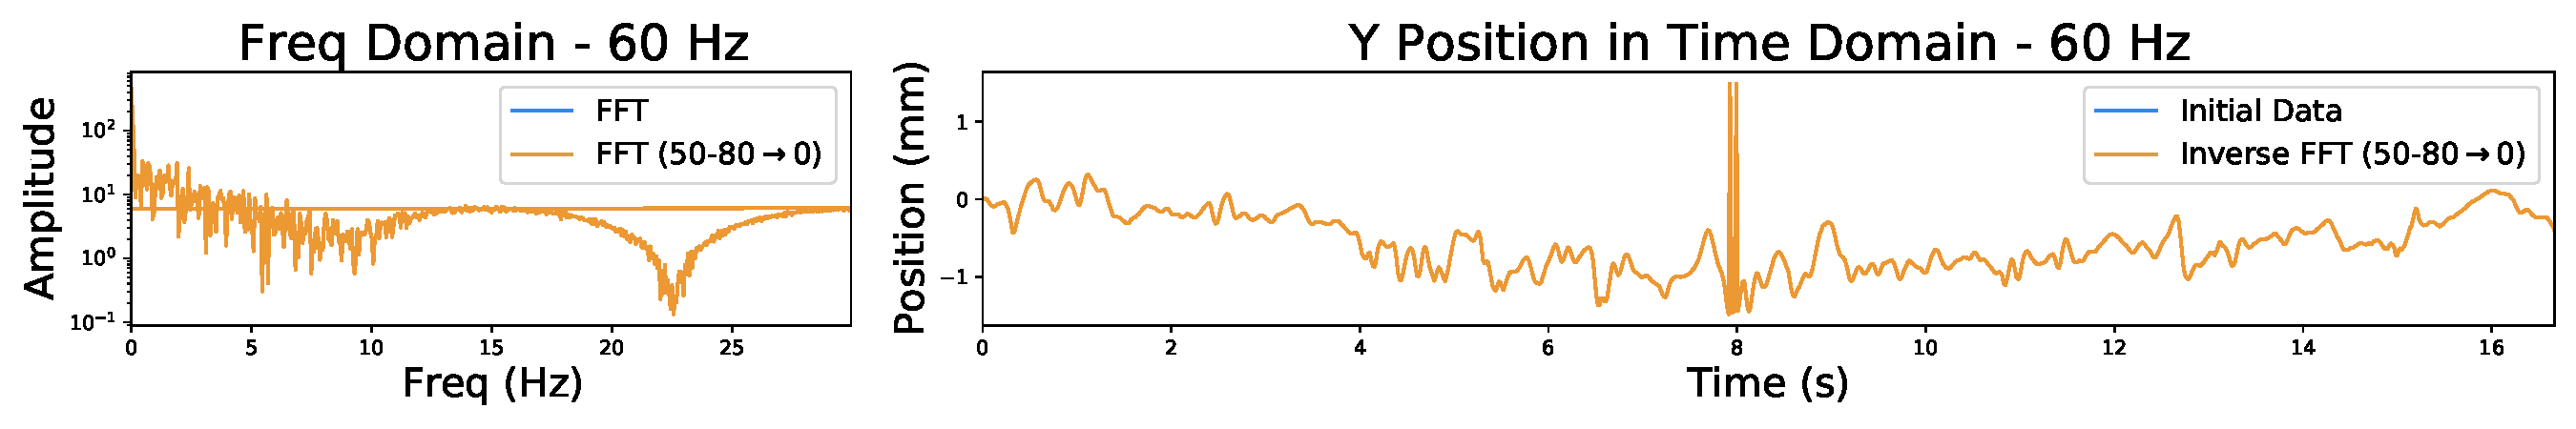
\includegraphics[width=\textwidth]{data_33_y_pos.pdf}
    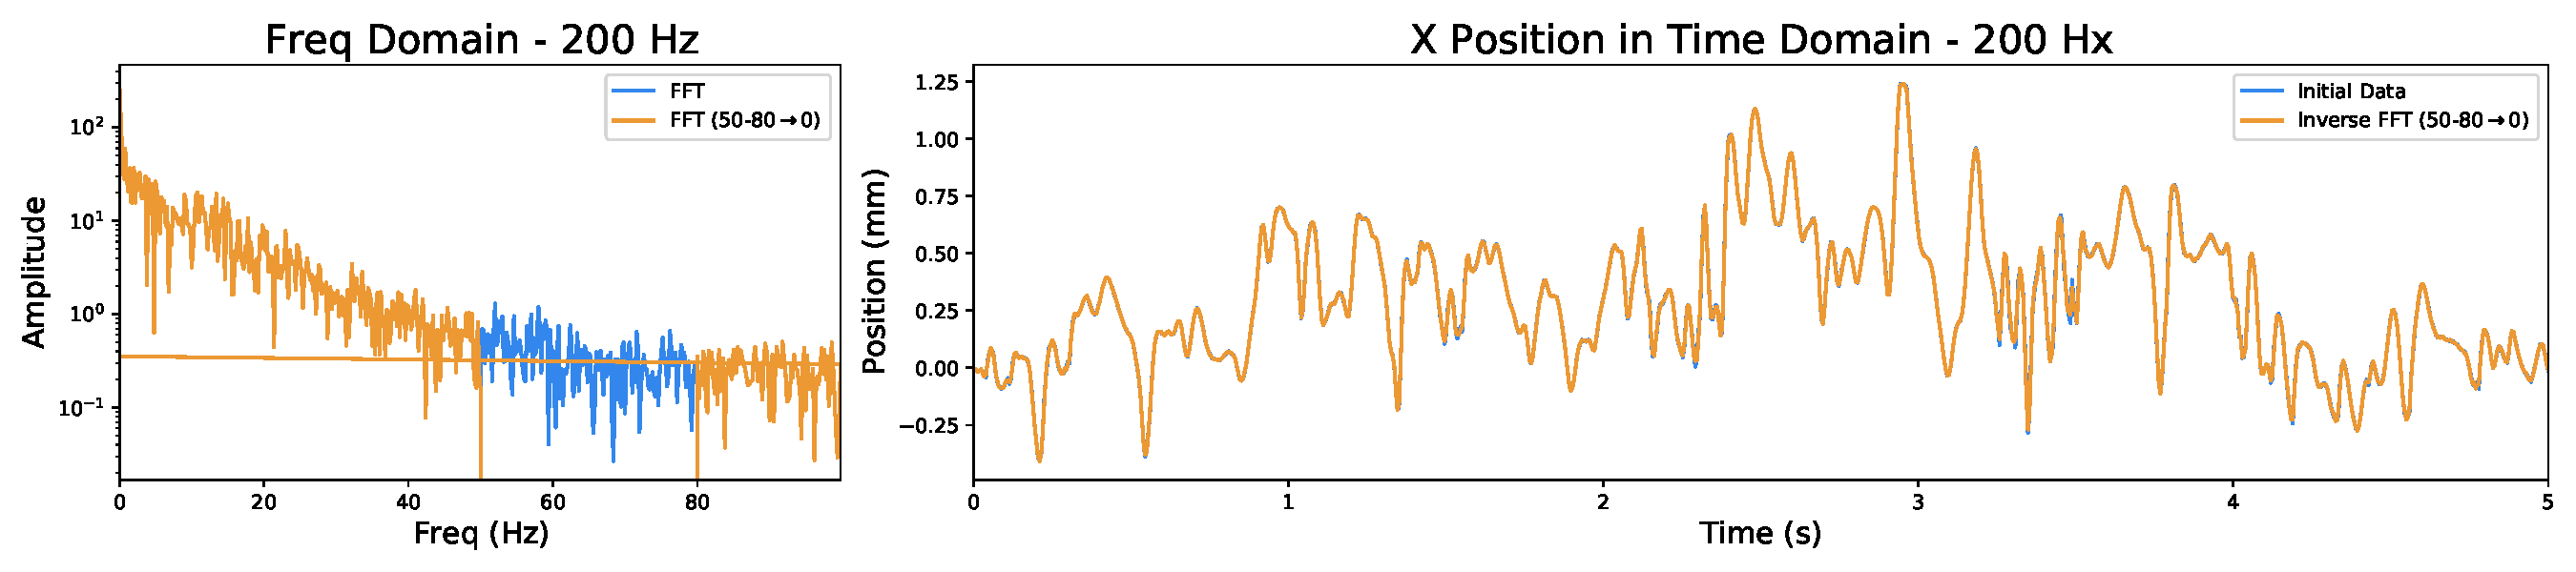
\includegraphics[width=\textwidth]{data_36_x_pos.pdf}
    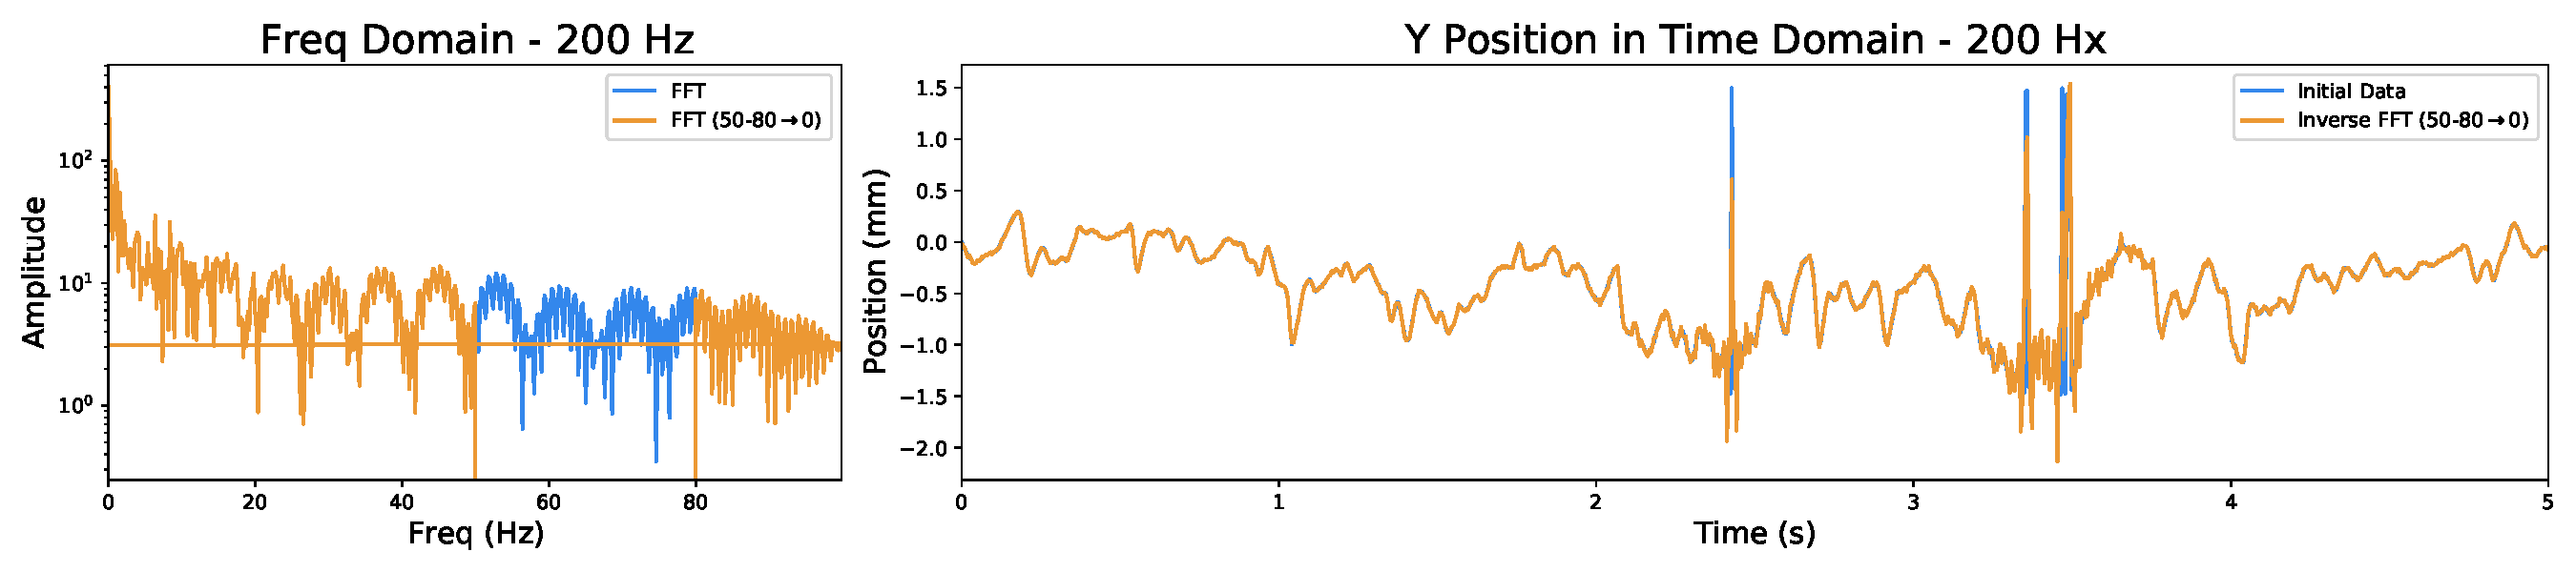
\includegraphics[width=\textwidth]{data_36_y_pos.pdf}
	\caption{Position data for the 60 and 200 Hz capture rate of the Bad Data. Both the X and Y data are shown here. Notice how odd the data looks in the frequency domain. This is a result of both the air currents and the possible error in capture rate.}
    \label{fig:flawed_pos}    
\end{figure}

\begin{figure}[!ht]
\centering
    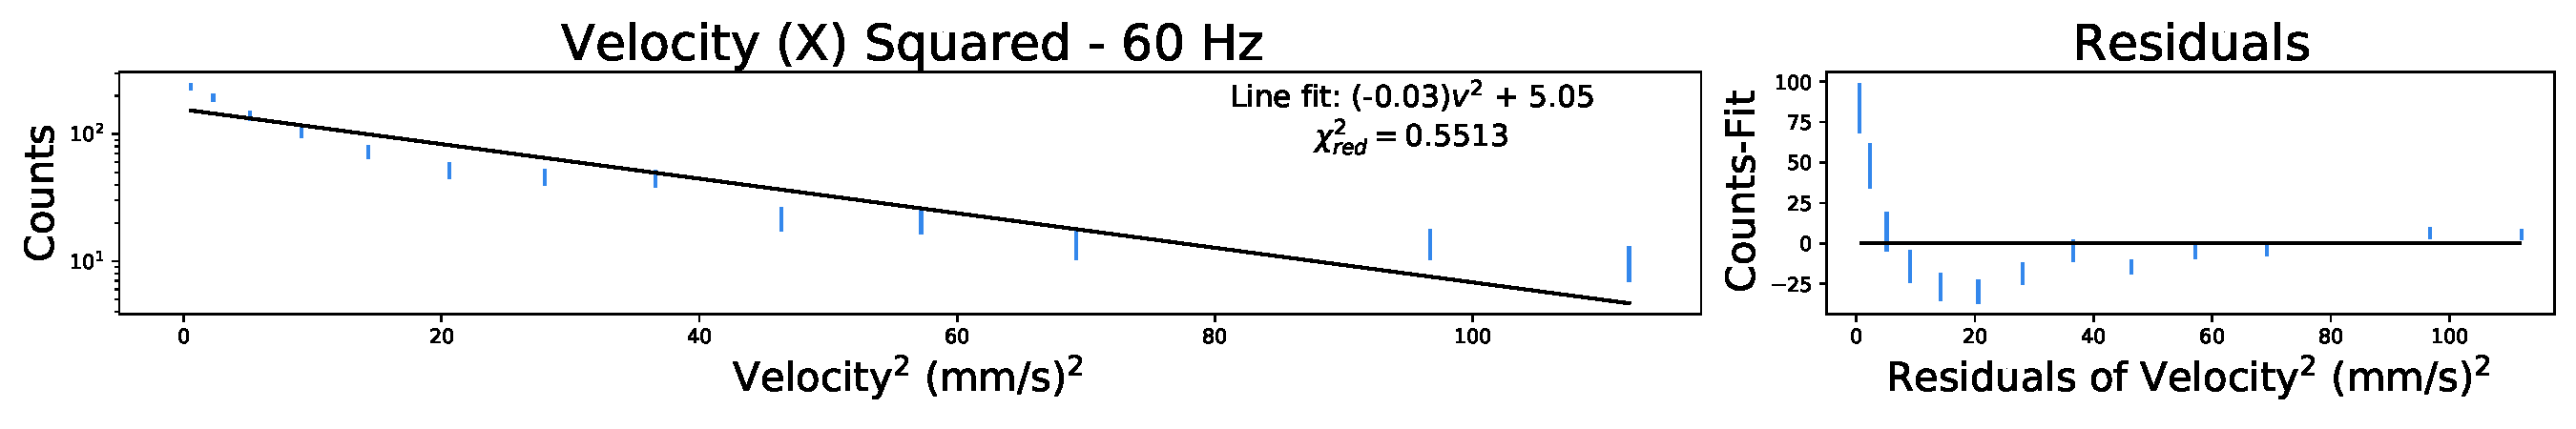
\includegraphics[width=\textwidth]{data_33_x_vel.pdf}
    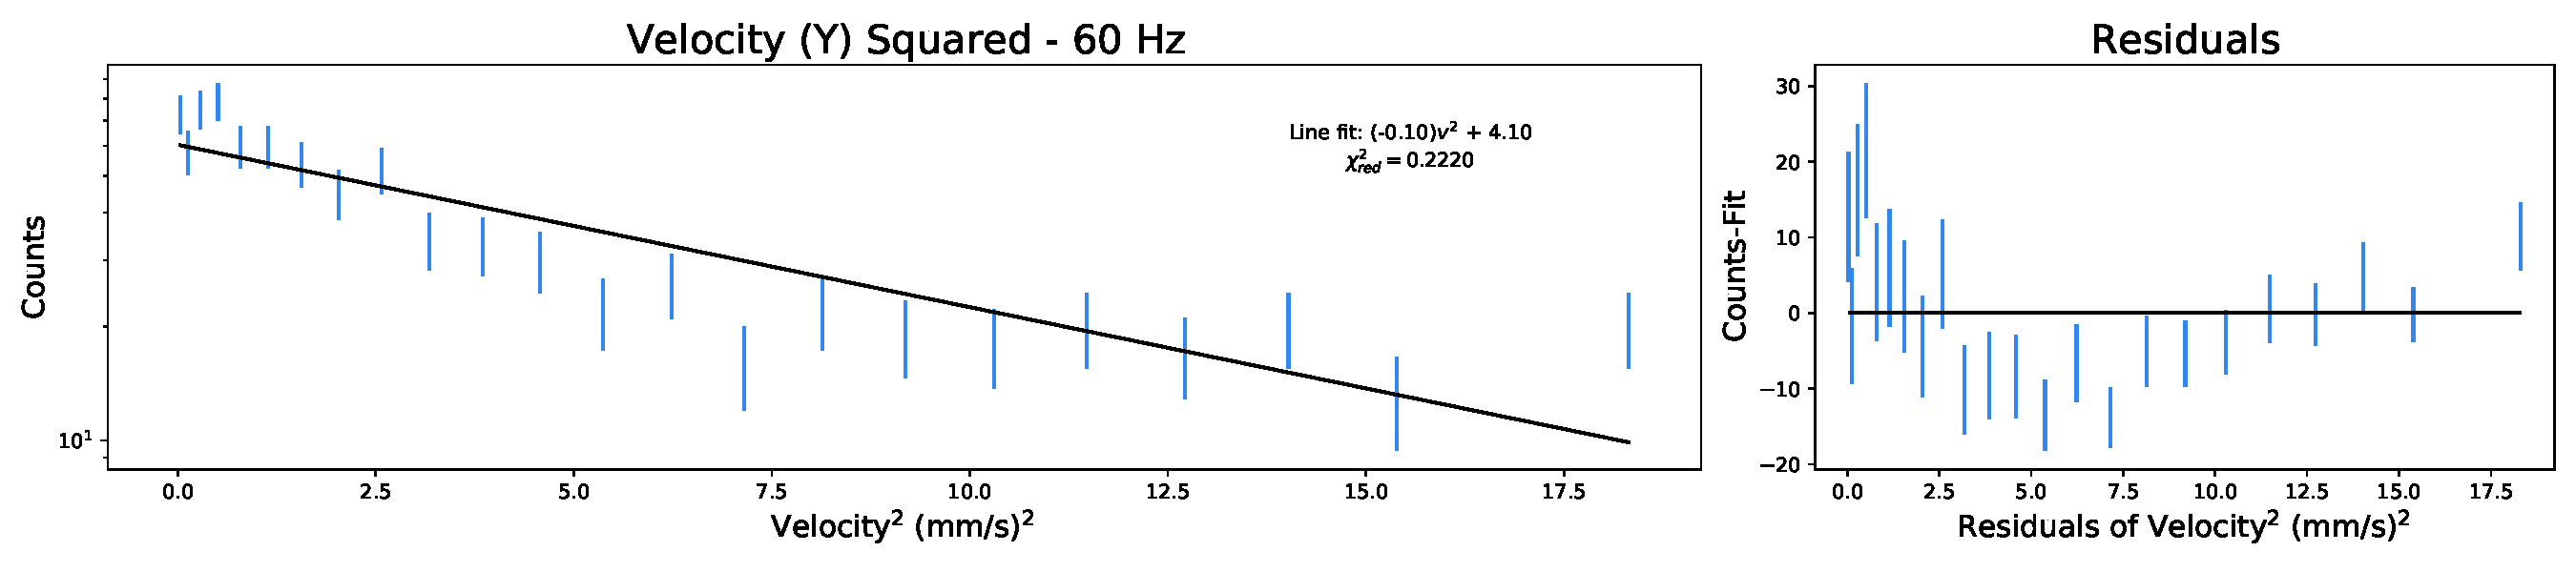
\includegraphics[width=\textwidth]{data_33_y_vel.pdf}
    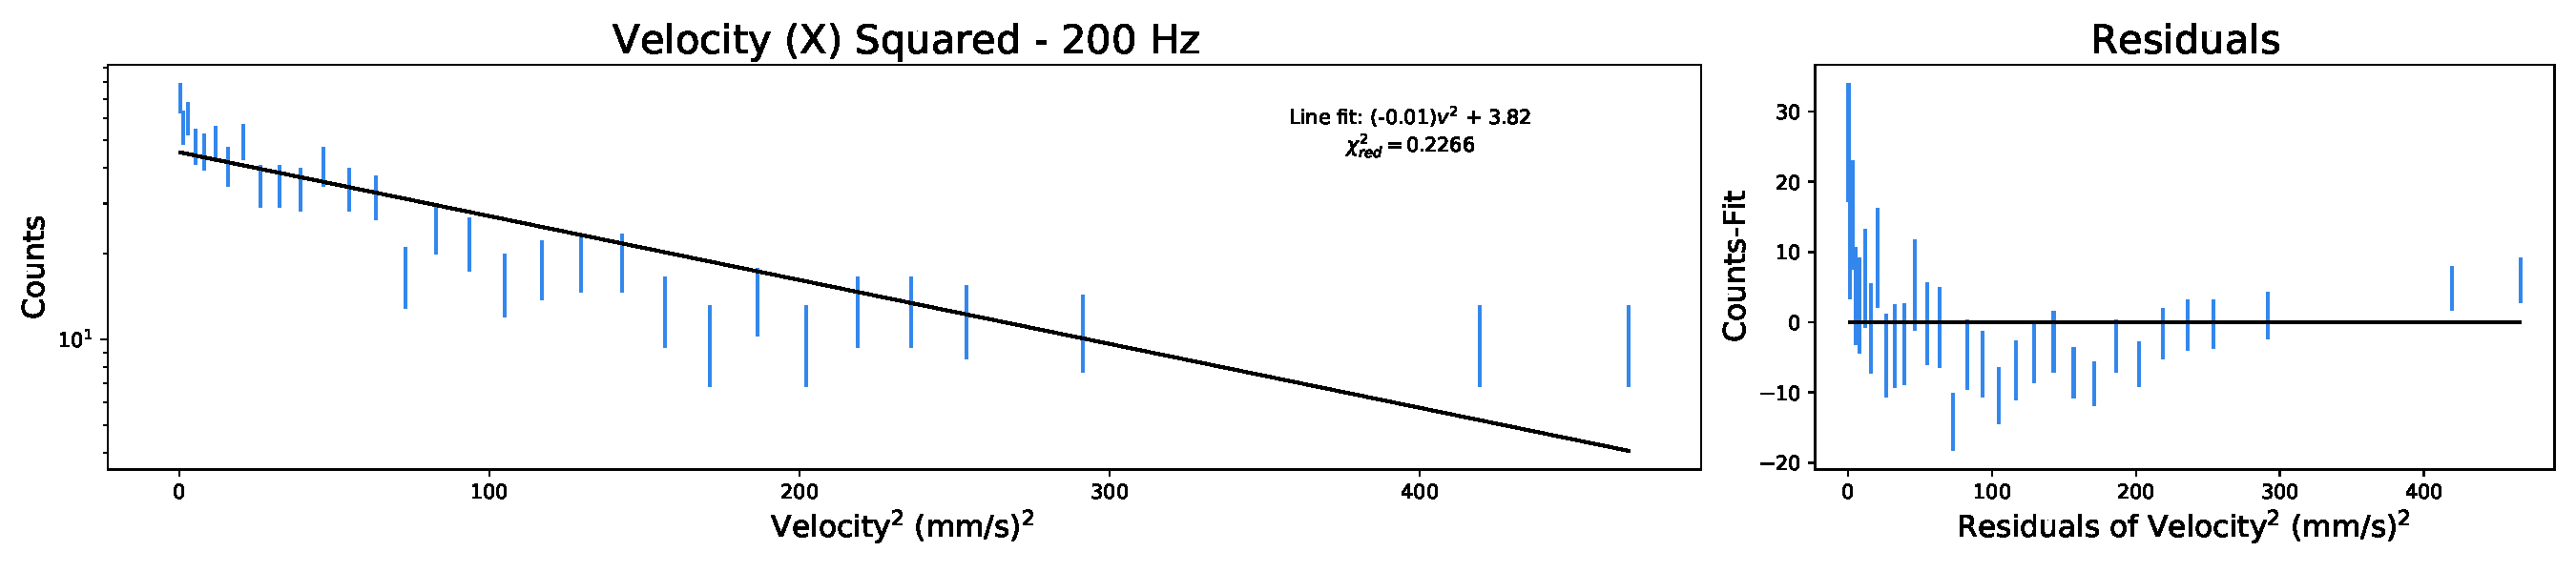
\includegraphics[width=\textwidth]{data_36_x_vel.pdf}
    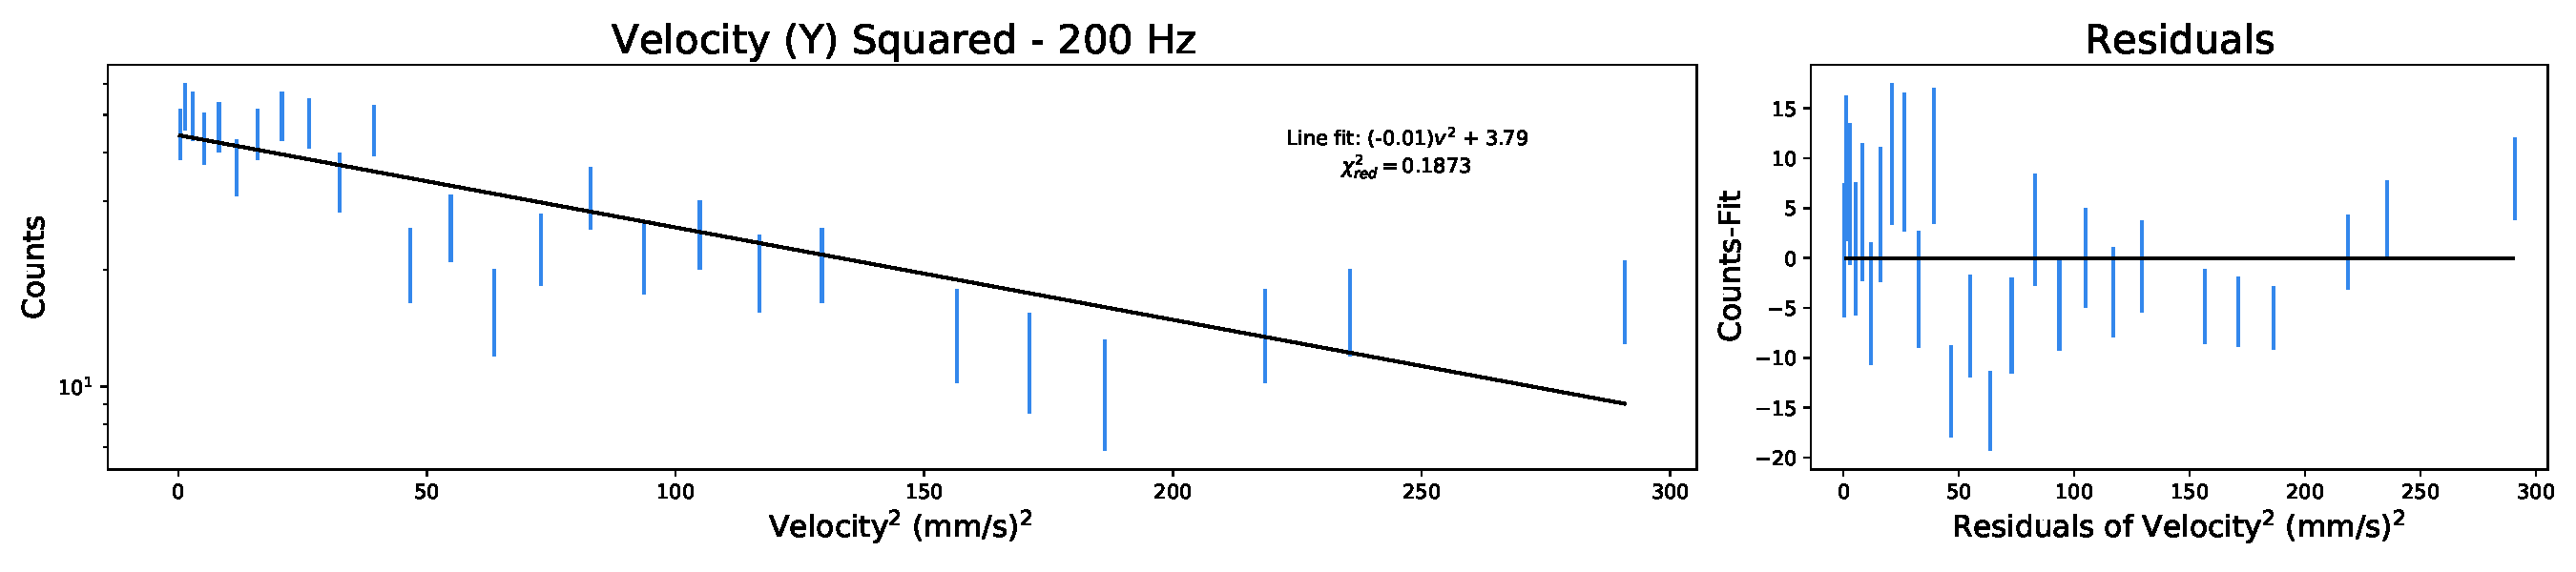
\includegraphics[width=\textwidth]{data_36_y_vel.pdf}
	\caption{Velocity data for the 60 and 200 Hz capture rate of the Bad Data. Both the X and Y data are shown here. The residual plots show how the exponential fit was not good for this data.}
    \label{fig:flawed_vel}
\end{figure}

The full analysis of the flawed data can be seen in Figures \ref{fig:flawed_pos} and \ref{fig:flawed_vel}. The characteristics seen here have little structures, and the analysis of the 200 Hz spectrum has a clear absence of the micro-motion is is expected to be seen. This point is what hints at the possibility that the data was not actually collected at the 200 Hz. The Y position data has a very odd behavior in the frequency domain that is best described by an oscillatory wind pattern, such as from the heating system, opening and closing of doors, or individuals walking past. None of these sources were observed during the data collection, so the data cannot be considered with those in mind. The source of this analysis is the same as for the usable data, so the nuances of the choices in the graphs will be described below.

The mass calculated with this data was sub picogram, with a larger varience according to the bin size used. Analyzing the X-velocity data, the 60 Hz capture gives a mass of $\approx 0.39 \pm 0.04$ pg and the 200 Hz capture gives a mass of $\approx 0.043 \pm 0.004$ pg (Figure \ref{fig:flawed_vel}). Analyzing the Y-velocity data, 60 Hz capture gives a mass of $\approx 0.81 \pm 0.09$ pg and the 200 Hz capture gives a mass of $\approx 0.045 \pm 0.006$ pg (Figure \ref{fig:flawed_vel}). All of these are abnormally small for the actual particle. When taken into account with extra kinetic energy from the wind pushing the particle around, the mass expected would be much lower than the actual mass of the particle. So, the fact that this method yielded a very small mass is reasonable.

\subsection{Analyzing Motion}
%% Give the analysis of motion, x and y
\begin{figure}[!ht]
\centering
    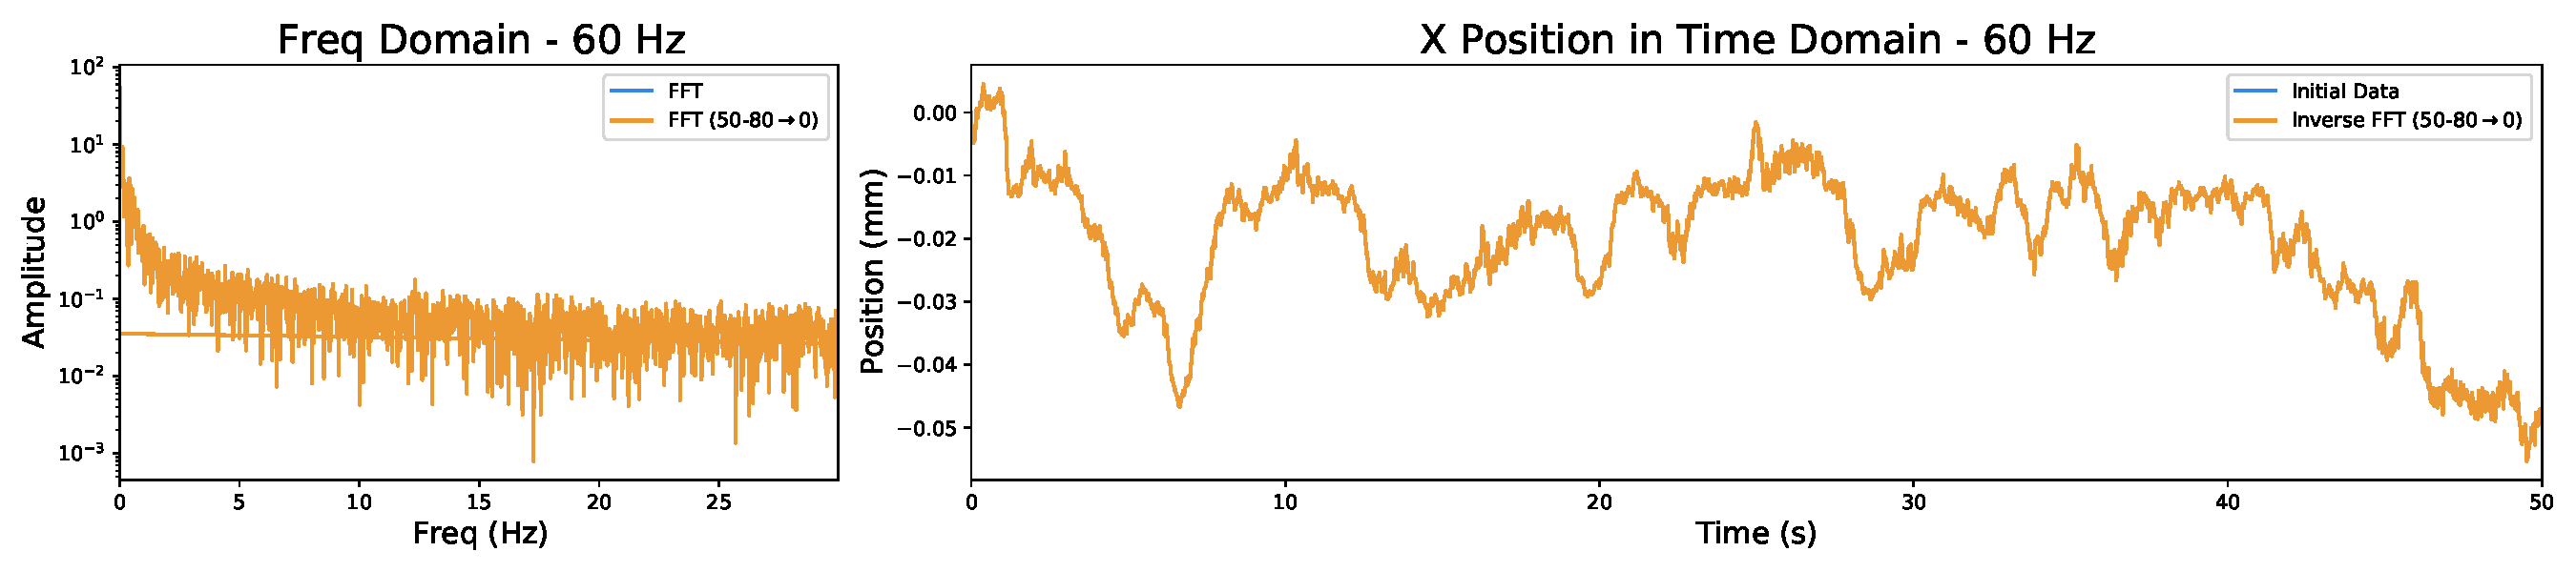
\includegraphics[width=\textwidth]{data_01_x_pos.pdf}
    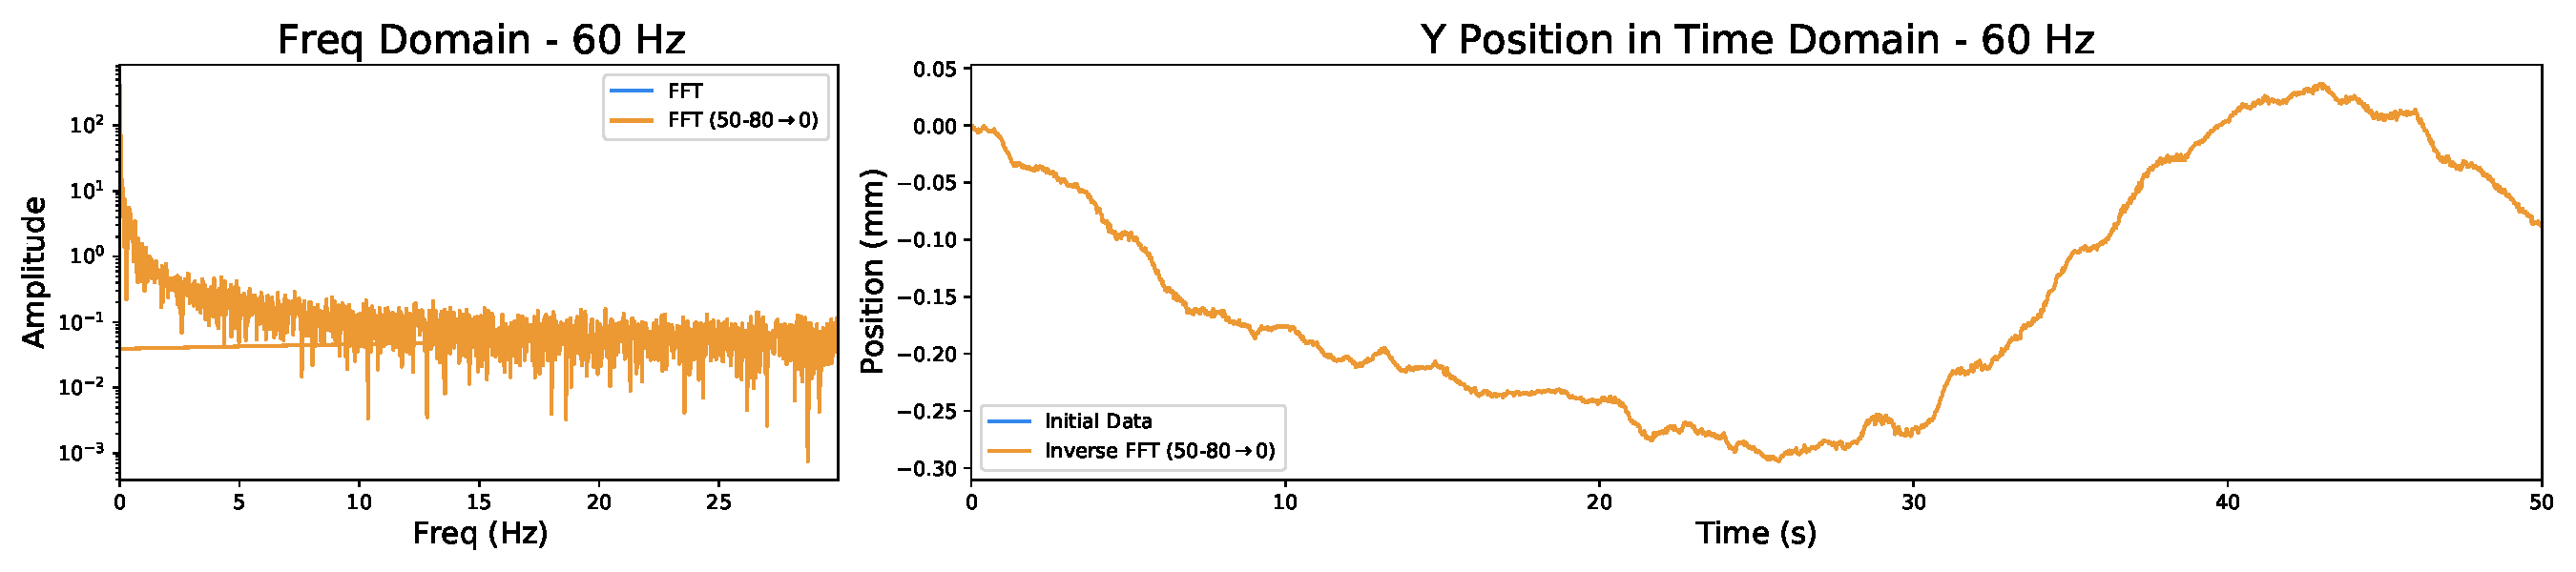
\includegraphics[width=\textwidth]{data_01_y_pos.pdf}
	\caption{The 60 Hz data of the Quality Capture. There seems to possibly be an overarching oscillation to the Y position data, possibly as the result of some air current.}
    \label{fig:01_pos}
\end{figure}

\begin{figure}[!ht]
\centering
    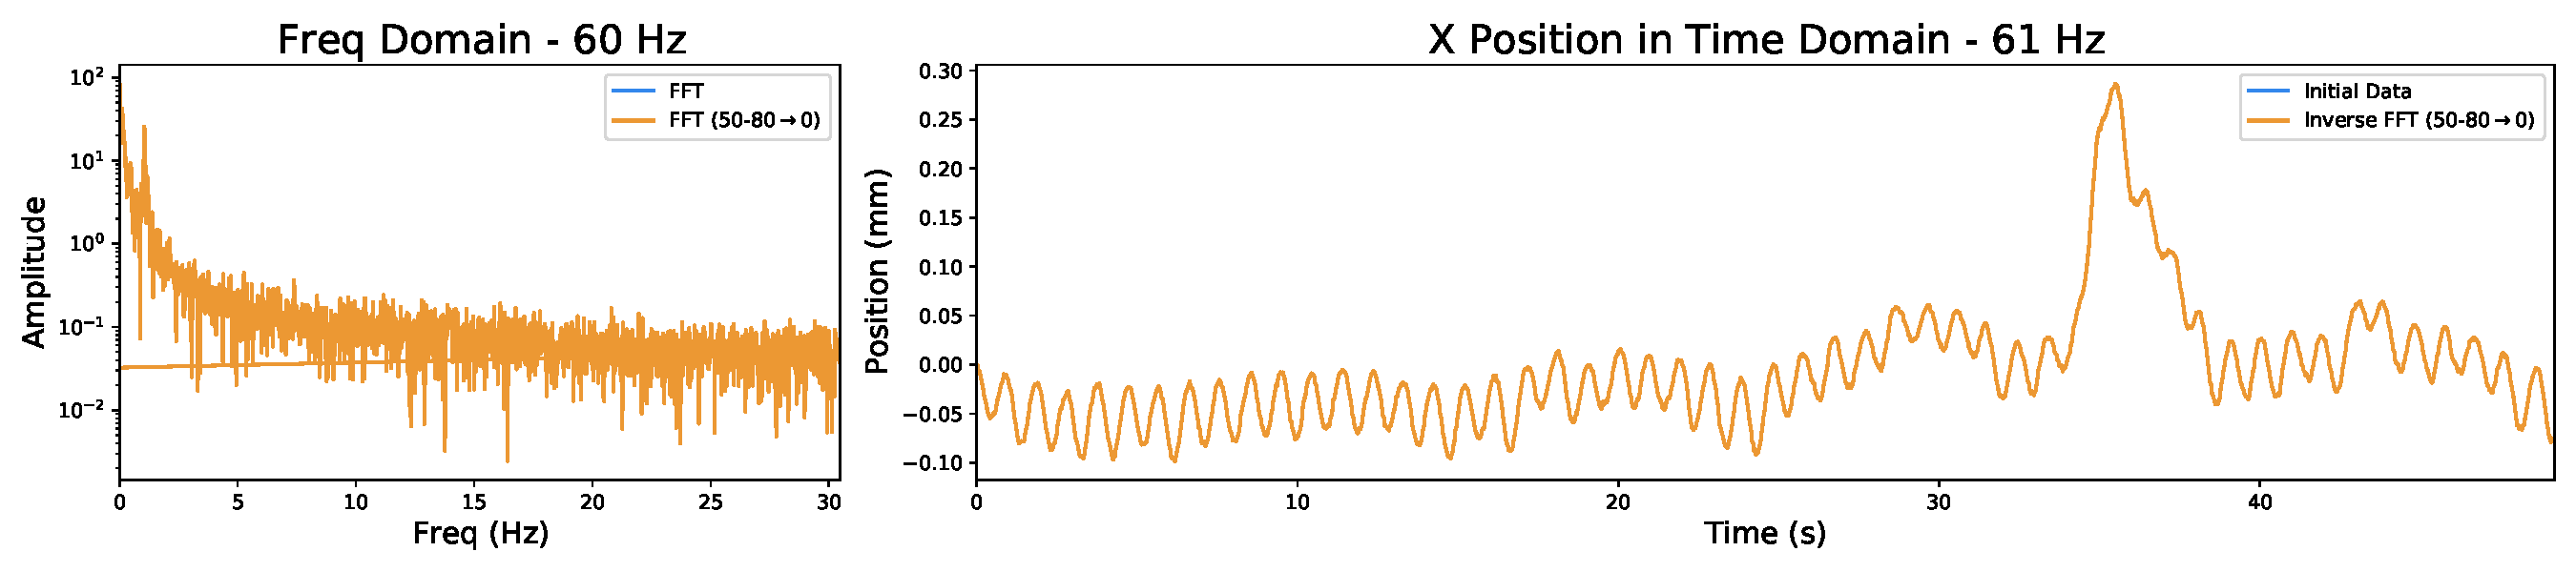
\includegraphics[width=\textwidth]{data_03_x_pos.pdf}
    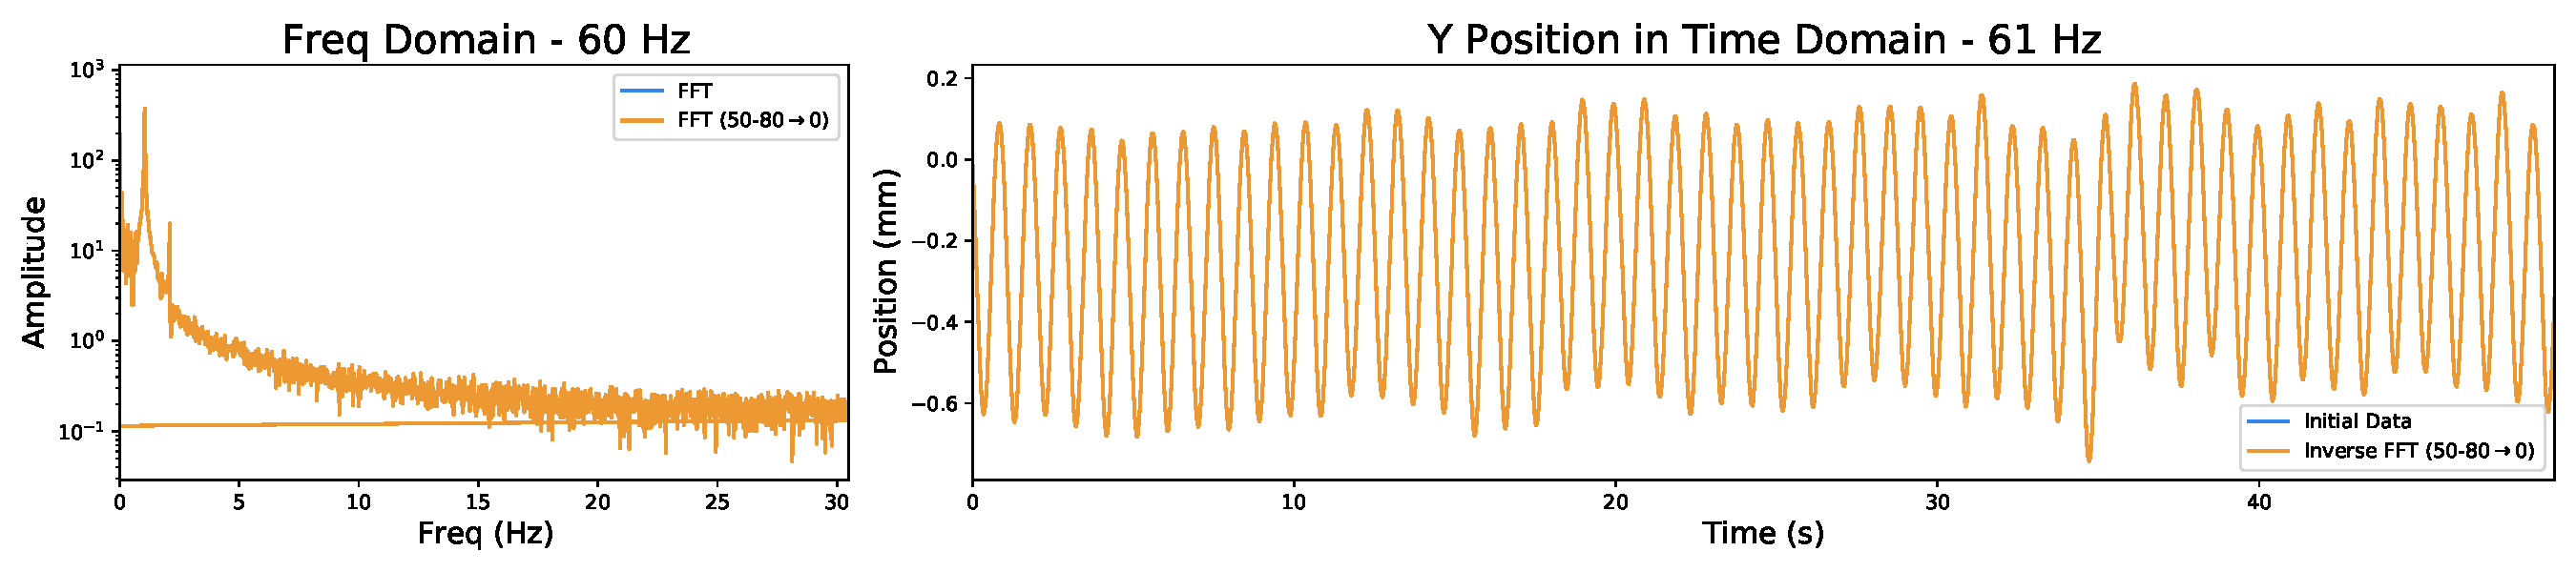
\includegraphics[width=\textwidth]{data_03_y_pos.pdf}
	\caption{The 60 Hz data of the Quality Capture. The presence of the 60 Hz micro-motion is evident.}
    \label{fig:03_pos}
\end{figure}

\begin{figure}[!ht]
\centering
    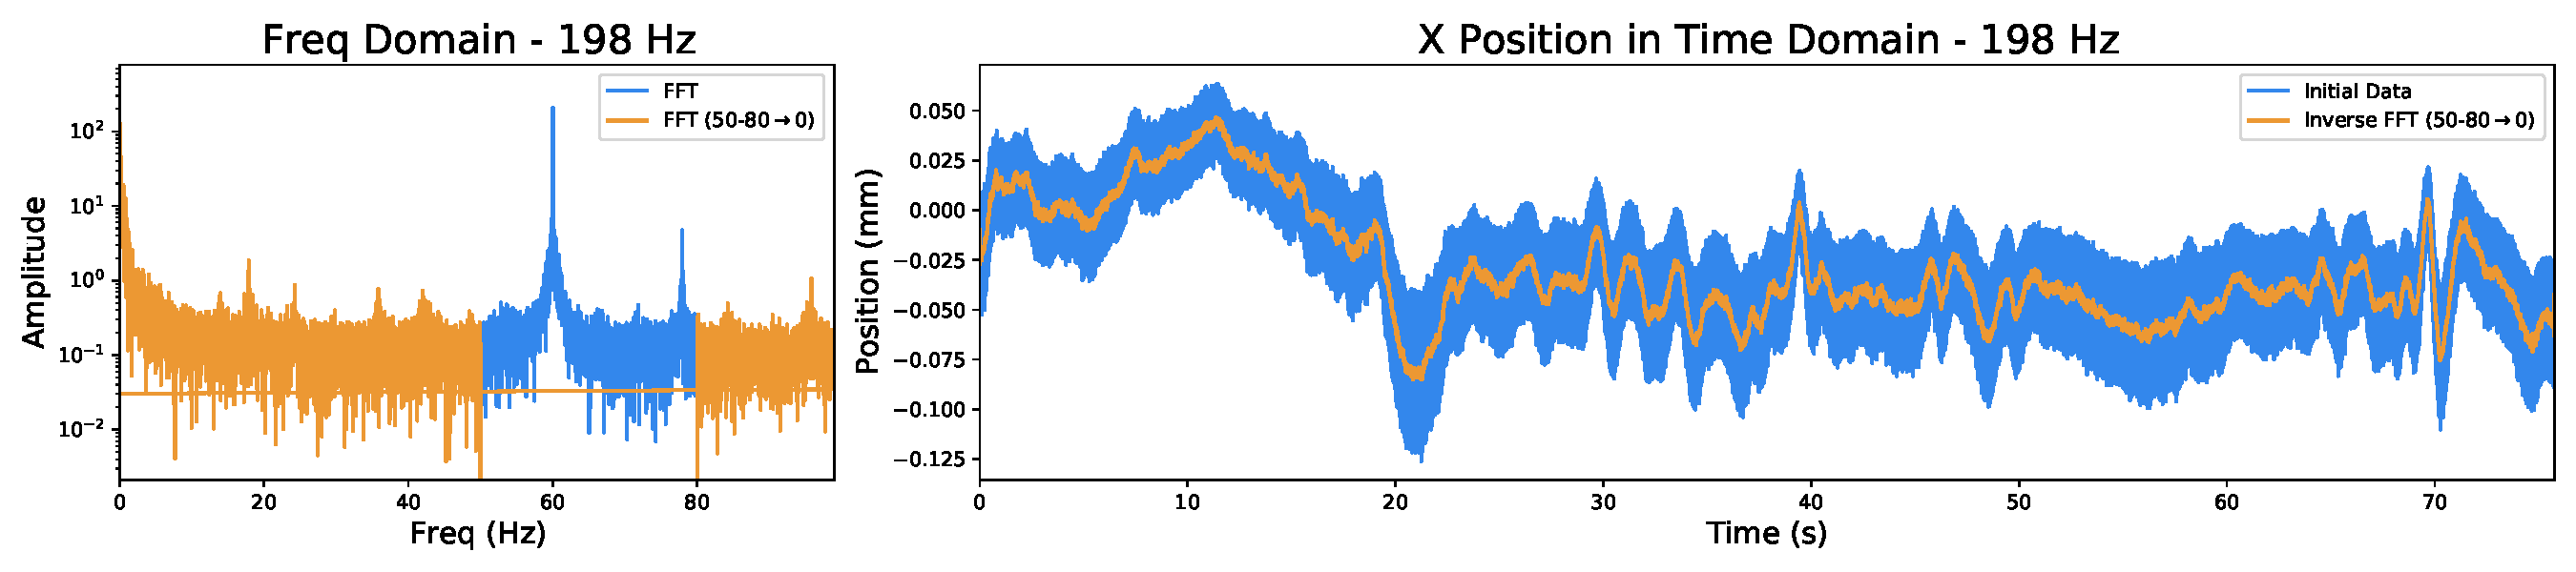
\includegraphics[width=\textwidth]{data_04_x_pos.pdf}
    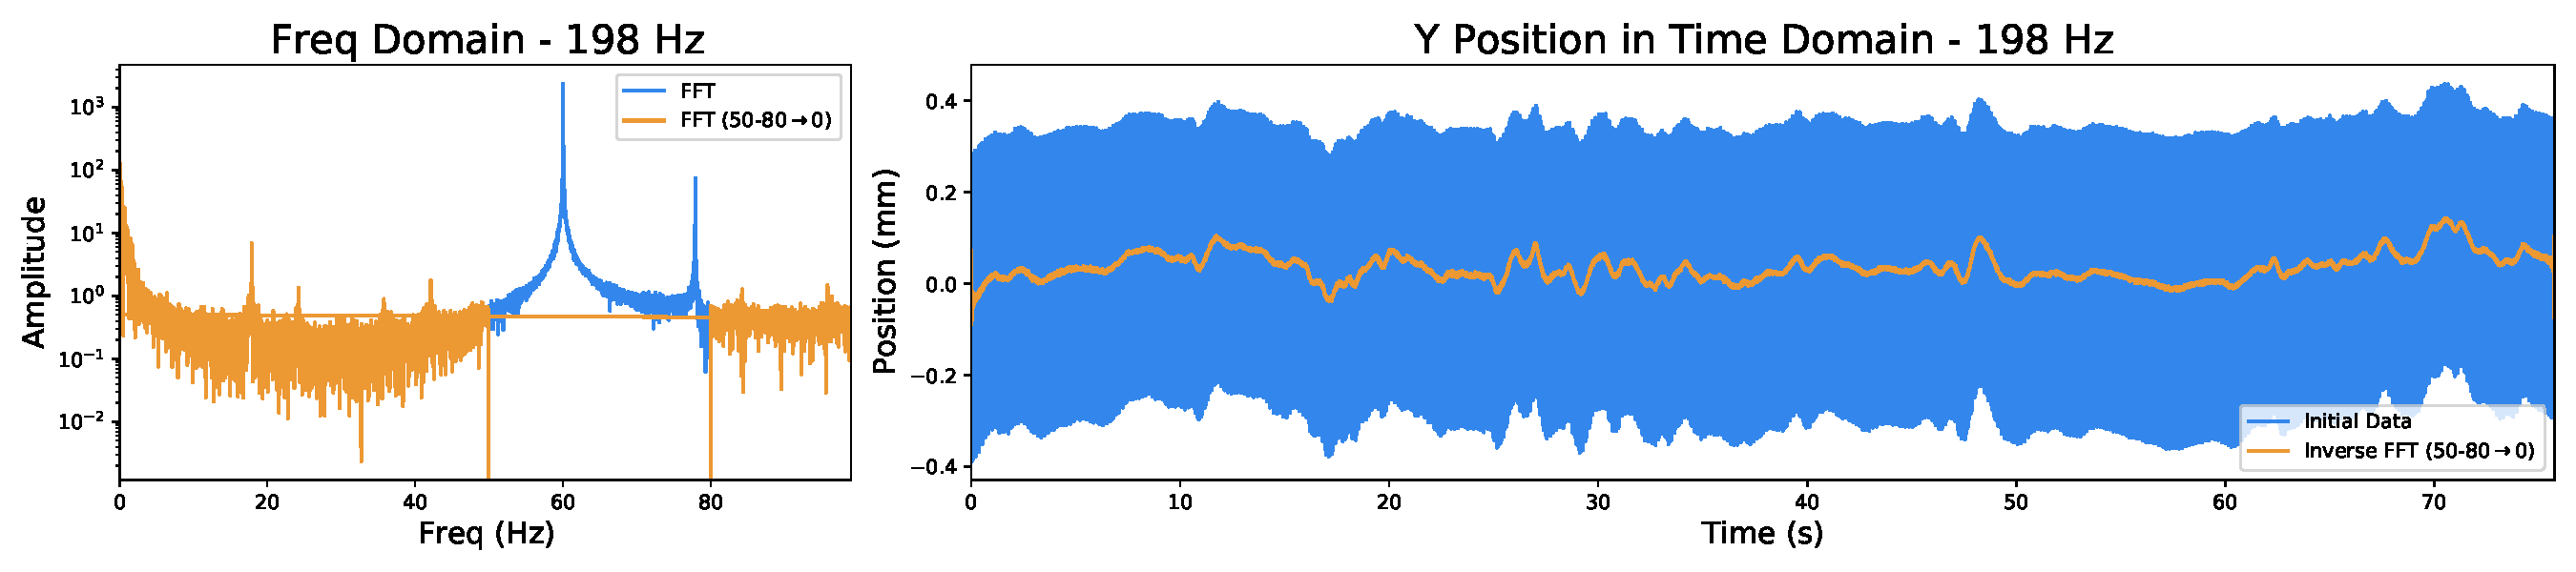
\includegraphics[width=\textwidth]{data_04_y_pos.pdf}
	\caption{The 198 Hz data of the Quality Capture. It can be seen how well the data is cleaned up once the 60 Hz and 78 Hz data are removed. }
    \label{fig:04_pos}
\end{figure}

For all of the data used, the images were passed through a ``cross-correlate\_simple.py" provided in lab and lightly modified to run the cross correlating algorithm more times, a total of 4 times, and all of the data. The code provides the x and y position of a detected particle in each frame, the x being horizontal (running parallel to the ground), and y being the vertical. The orientation of the paul trap was verticle, so it is expected that the micromoation should be in the Y-direction. Because of the orientation of the camera and the nature of using a circular Paul Trap, the micro-motion can also be seen in the X-direction. The X and Y positions of the particles with respect to have been plotted. Each was then transformed to the Fourier domain and the two peaks from the micro-motion, the 60 Hz and the 78 Hz peaks were set to 0. Then the data was transformed back to the time domain. This obviously worked for the 198 Hz data, but for the 60 Hz and 61 Hz data, their Niquest frequency is around 30 Hz, so the analysis provided no new information. Looking at Figure \ref{fig:04_pos}, the removal of the micro-motion cleaned up the evident motion due to everything else: air-currents and thermal fluctuations. To Attempt to find any air currents, any clear peaks in the Fourier domain can be analyzed to figure out the source. If a oscillatory source of noise, such as a heating unit or a shaking table, were present they could be subtracted at this time. However, there didn't seem to be any other clear sources of noise, so it will be assumed that all of these flucuations are from the thermal energy of the particle. 

Looking at the 60 Hz data, there seems to be a clear drift in teh location of the particle over time in the Y direction (Figure \ref{fig:01_pos}), but in the X direction the walking seems to be more random (Figure \ref{fig:01_pos}). In the 61 Hz data there is a clear osscilation, something above the frequency the data was taken at. It's clear that the source of this oscilation was the mirco-motion. The reason that the 60 Hz didn't pick up the same characteristic is because the frame rate is at the same speed as the oscilations of trap, effectively always taking a picture of the particle at the same position in the overpowering wave. 

\subsection{Analyzing Velocity}
%% Give the analysis of velocity
\begin{figure}[!ht]
\centering
    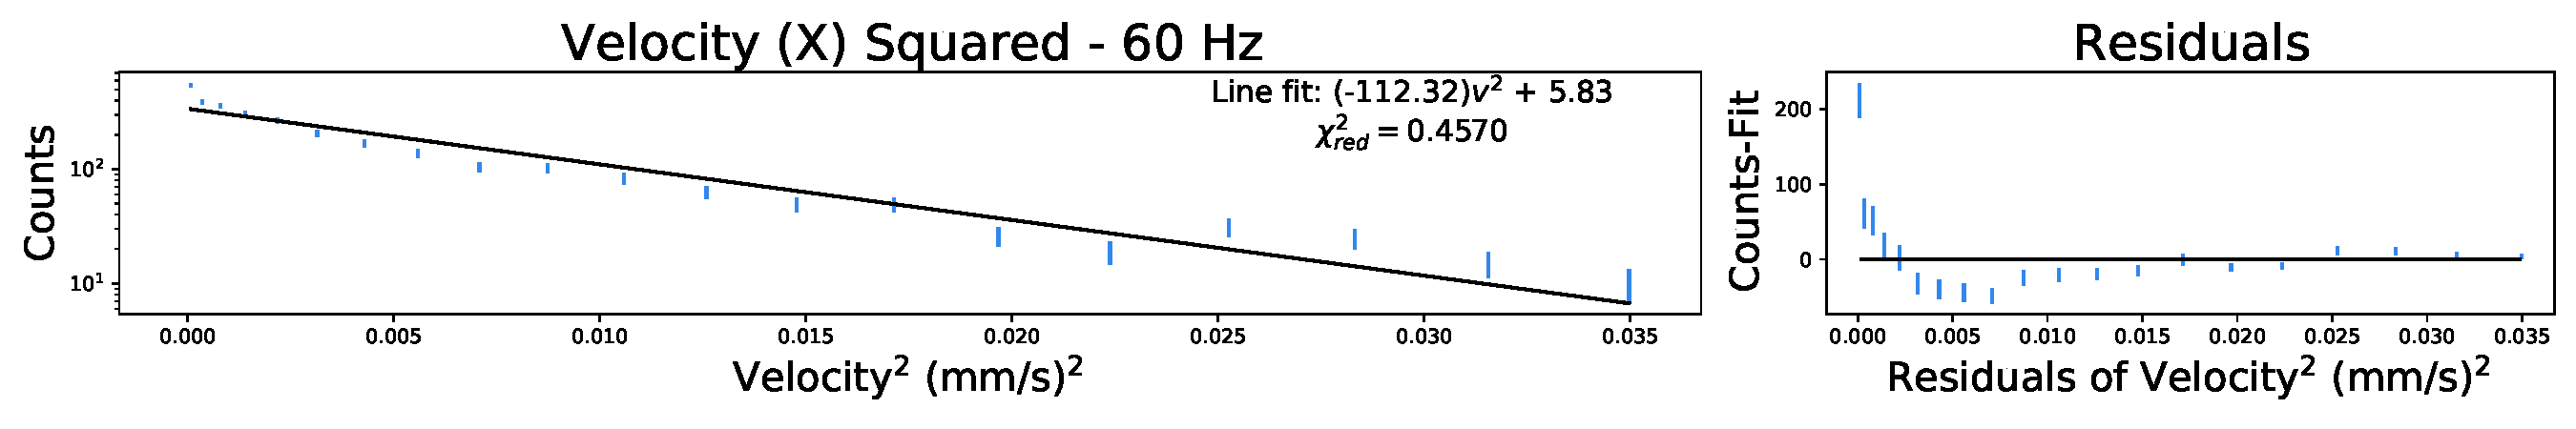
\includegraphics[width=\textwidth]{data_01_x_vel.pdf}
    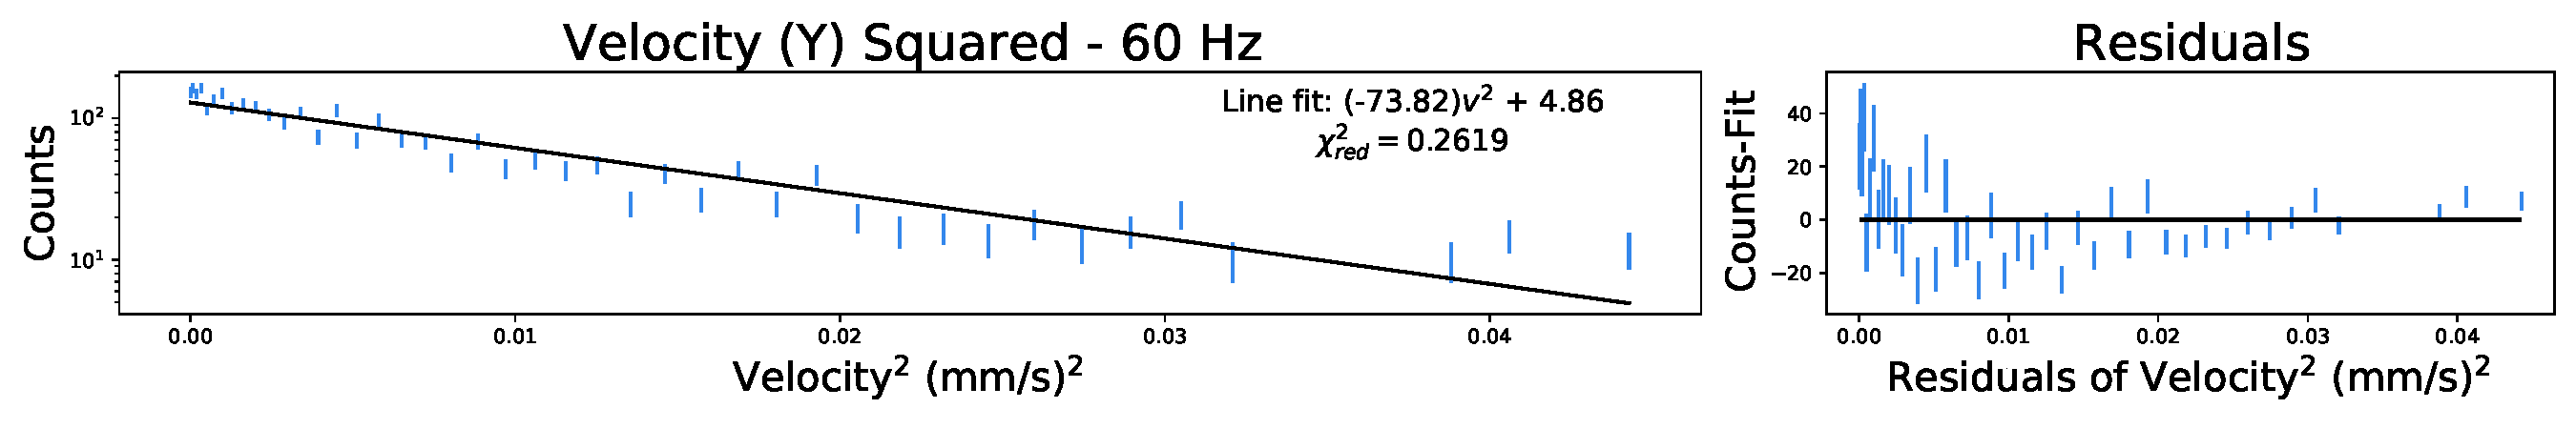
\includegraphics[width=\textwidth]{data_01_y_vel.pdf}
    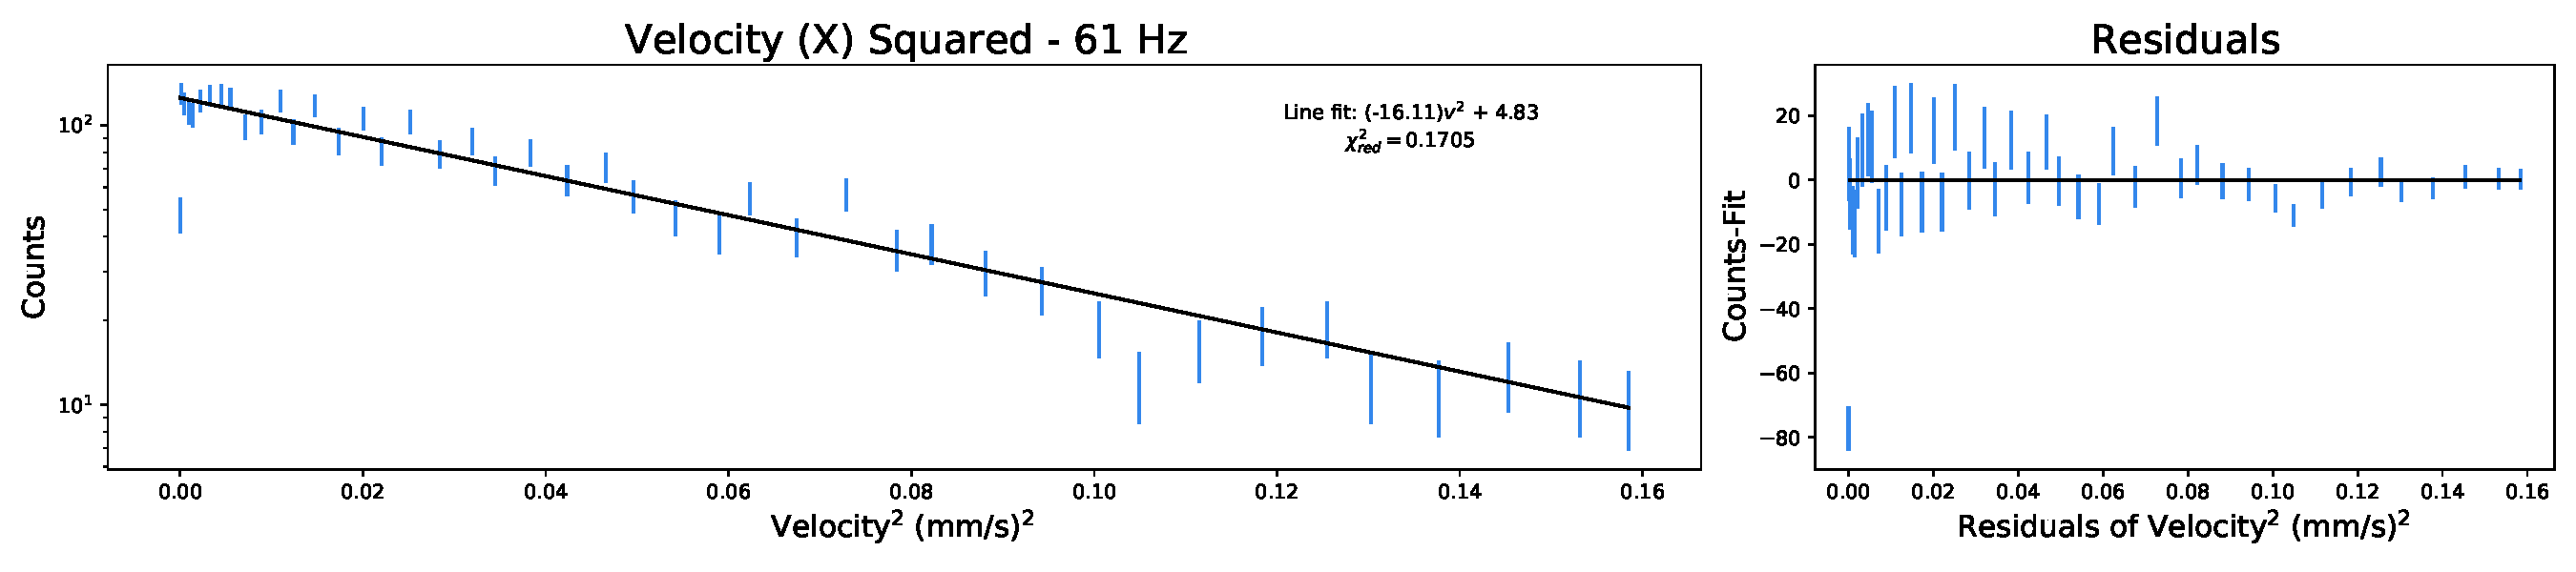
\includegraphics[width=\textwidth]{data_03_x_vel.pdf}
    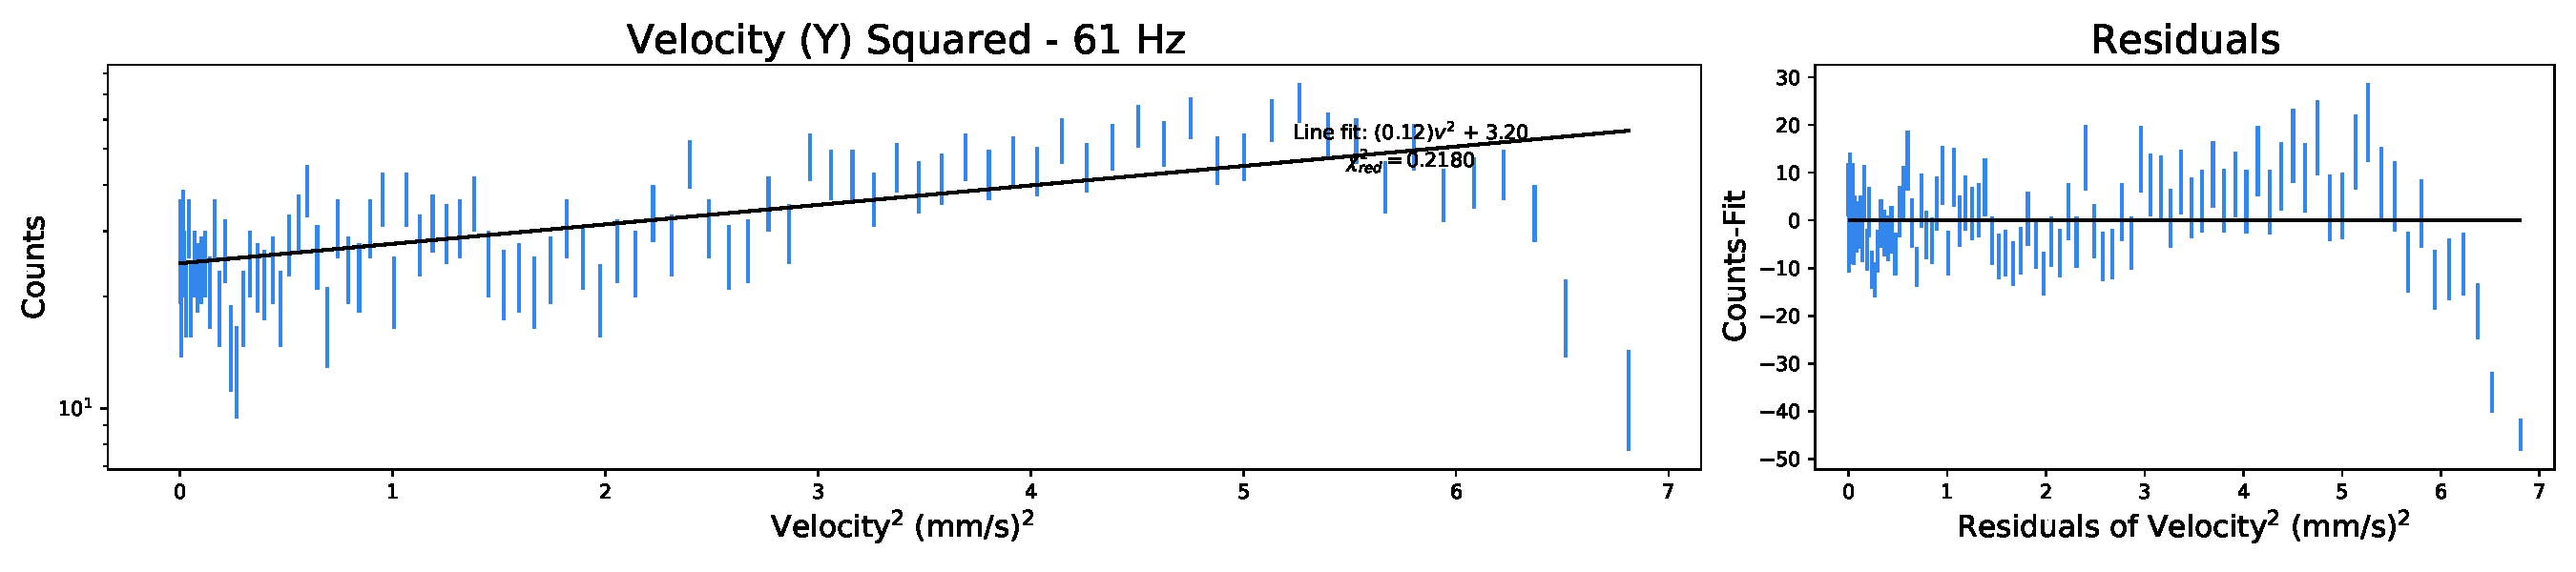
\includegraphics[width=\textwidth]{data_03_y_vel.pdf}
	\caption{The velocity histograms for both the X and Y direction of the 60 and 61 Hz captures. The residuals show that, while both the fits may look okay to the left, there is still an underlying physics to the setup.}
    \label{fig:low_hz_vel}
\end{figure}

\begin{figure}[!ht]
\centering
    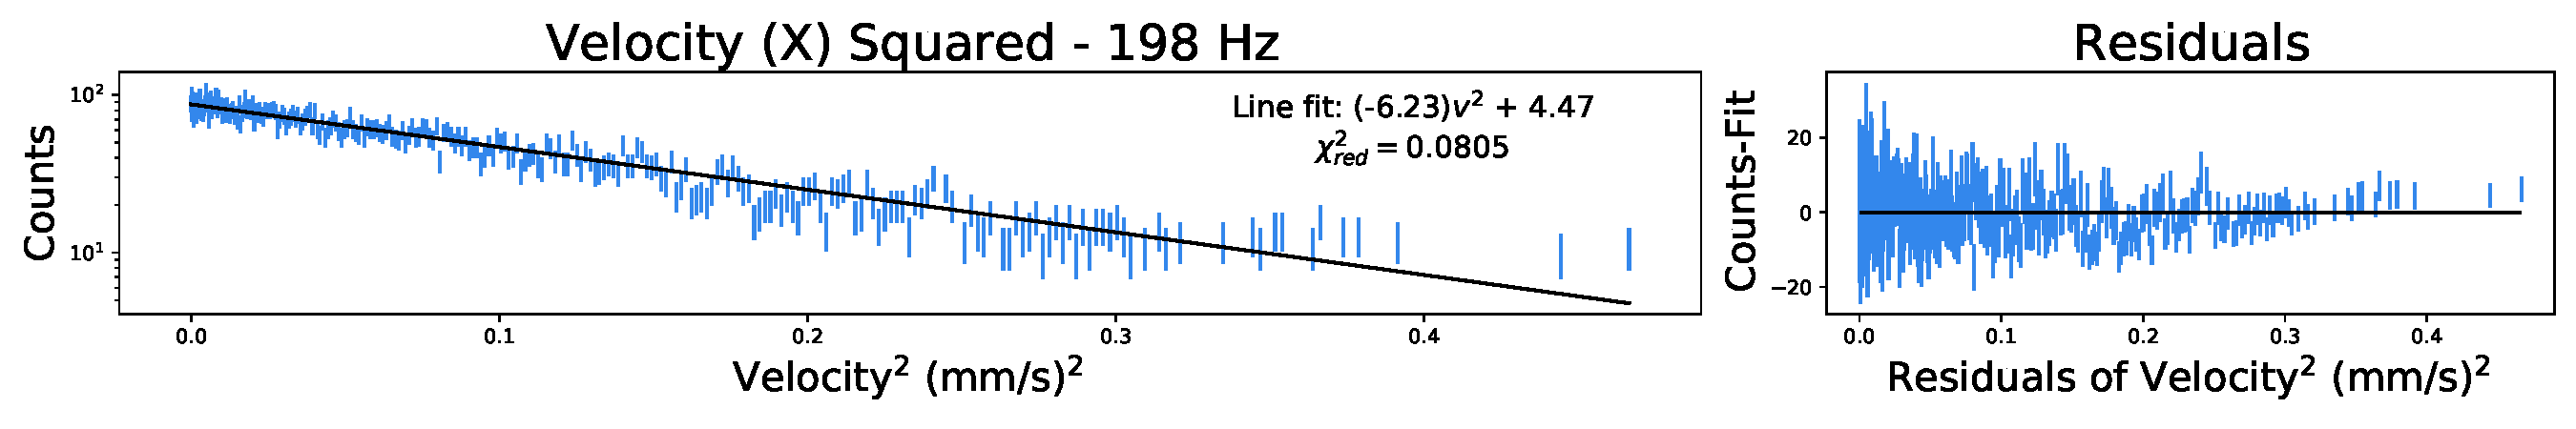
\includegraphics[width=\textwidth]{data_04_x_vel.pdf}
    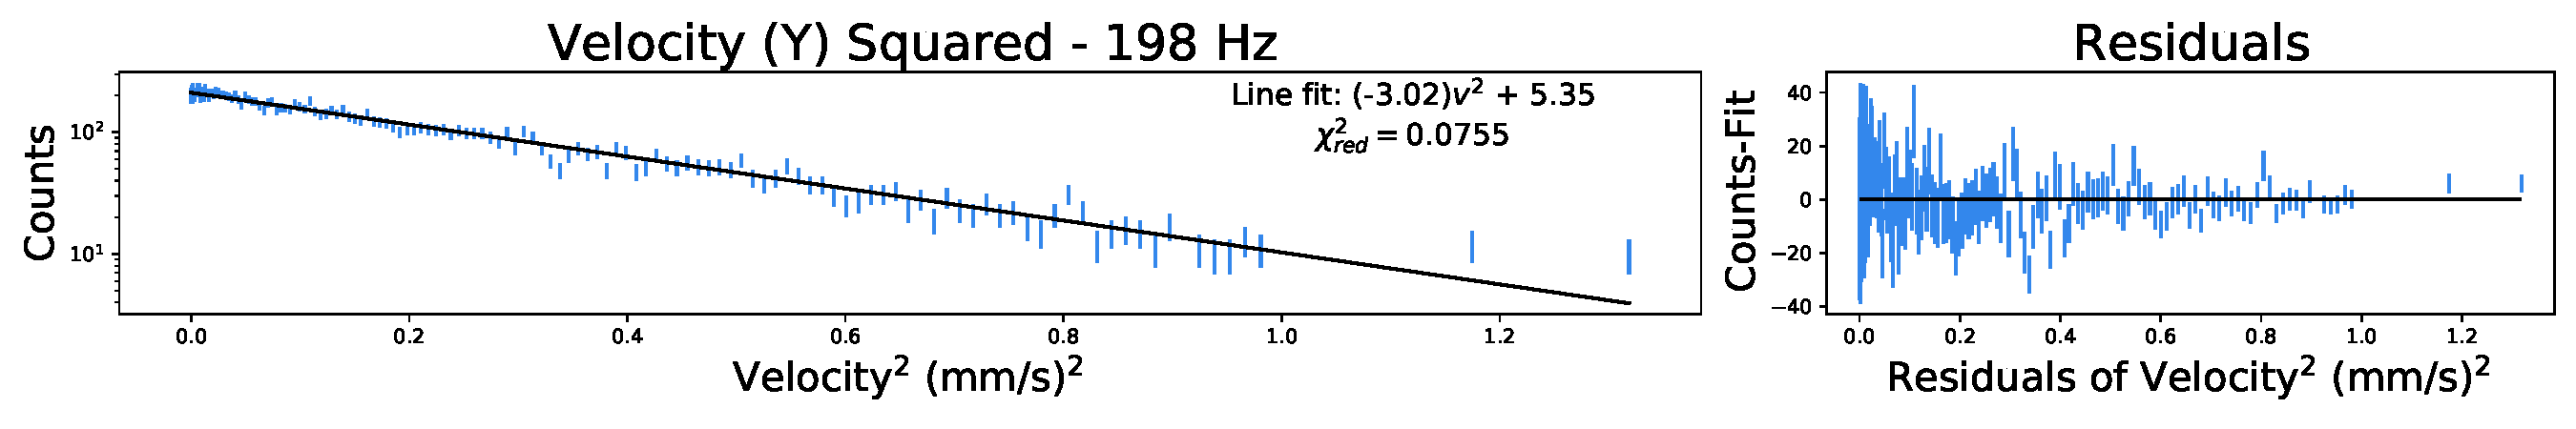
\includegraphics[width=\textwidth]{data_04_y_vel.pdf}
	\caption{The velocity histograms of the 198 Hz capture. The residuals show very good characteristics and seem to point that this is the correct interpretation.}
    \label{fig:high_hz_vel}
\end{figure}

To get an estimate of the speed of the particle in the trap as a function of time two consecutive frames can be subtracted and can be divided by the difference in time between the two frames. This evolution of velocities can then be looked at as a histogram, instead of a time plot. The realm of error analysis can now be estimated as a Poisson distribution, assuming that the error from the ``cross-correlate\_simple.py" is much smaller than that given by Poisson: the square root of the number of items in a given bin. All bins that had less than 10 data points in them were removed from the analysis, as at the regime the Poisson distribution starts to break down. This analysis gives a rough estimate for the probability that the particle is traveling at a given speed. Using Eq \ref{eq:marg_prob2}, a linear fit can be applied to the natural log of the square of the right edge of the velocity bins. The slope will then be equal to $-\frac{m}{2 k_B T}$ and can be used to analyze the mass. 

It is interesting to look at how the inability to remove the micro-motion from the 61 Hz catpure added a clear leveling off to the velocities (Figure \ref{fig:low_hz_vel}). The positive slope seen should give a negative mass as well. The general take away is that the characteristics seen are not useful in this specific analysis. Interestingly, the 60 Hz data is still well behaved and gives a reasonably possible slope. Looking at the residuals of all three of the data collections (Figures  \ref{fig:low_hz_vel} and \ref{fig:high_hz_vel}), it is clear which have reasonable linear fits, and which have underlying physics from the micro-motion that has not been addressed. 


\subsection{Calculating Mass}
%% Give the calculated mass, for all of them - provide source of error bar

Assuming that the temperature of the room was average room temperature (298.15 K), the mass can be calculated. The error was calculated by taking the resulting error in the slope given according to the error bars provided by the assumption of the dominance of the Poisson error. Depending on the number of bins used to characterize the data, the slope shifted slightly. A combination of visual justification and looking at the reduced $\chi^2$ value guided the correct number of bins to use. In the process of looking at the $\chi_\text{red}^2$, the value only neared 1 when the fit portrayed odd behavior, from either radically small bins or not enough bins to have a good number of data points. This comes from the fact that the error bars are just an estimate of what they should be. So, the aim of the $\chi^2$ value was around $0.01-0.2$, depending on the graph. The calculated mass for each of the trials can be seen in Table \ref{tab:masses}.\footnote{All the data collected on the different bins can be found in \textbf{Appendix A} in Table \ref{tab:calc_data}}

\begin{table}[ht]
\caption{}
\label{tab:masses}
\centering
\begin{tabular}{lllll}
\multicolumn{5}{c}{{\ul Bad Data}}                                    \\
Freq   & Axis & Num of Bins & Mass (pg)         & $\chi_\text{red}^2$ \\ \hline
60 Hz  & X    & 100         & $0.39 \pm  0.04$  & 0.233               \\
       & Y    & 1000        & $0.81 \pm 0.09$   & 0.222               \\
200 Hz & X    & 100         & $0.043 \pm 0.004$ & 0.227               \\
       & Y    & 1000        & $0.045 \pm 0.006$ & 0.187               \\
       &      &             &                   &                     \\
\multicolumn{5}{c}{{\ul Quality Data}}                                \\
Freq   & Axis & Num of Bins & Mass (pg)         & $\chi_\text{red}^2$ \\ \hline
60 Hz  & X    & 35          & $925 \pm 63$      & 0.457               \\
       & Y    & 35          & $523 \pm 46$      & 0.726               \\
61 Hz  & X    & 200         & $133 \pm 7$       & 0.170               \\
       & Y    & 100         & $-0.99 \pm 0.12$  & 0.218               \\
198 Hz & X    & 2000        & $51.3 \pm 0.8$    & 0.081               \\
       & Y    & 5000        & $24.8 \pm 0.3$    & 0.075              
\end{tabular}
\end{table}

From the calculations of the Quality Data, it would seem that the mass of the trapped particle is somewhere between thousands of picograms to tens of picograms. Considering that the 60 Hz data was collected at a lower frame rate and may not have accounted for the 78 Hz noise, of an origin that is not perfectly clear, that the 198 Hz value of tens of picograms should be considered as the measured mass. In considering the X or Y directional values, it's proposed that the Y value be taken. In an ideal trap, all of the micro-motion would be in the Y-direction. Obviously, that is not the case here. However, looking at the X-directional data (Figure \ref{fig:04_pos}), there seems to be a driving force present at a couple points in the time. The micro-motion detected in the Fourier domain is a full magnitude smaller. For this reason, the $24.8 \pm 0.3$ pg is the most reasonable mass to conclude. 

\subsection{Transient Response}
%% Give the transient response
\begin{figure}[!ht]
\centering
    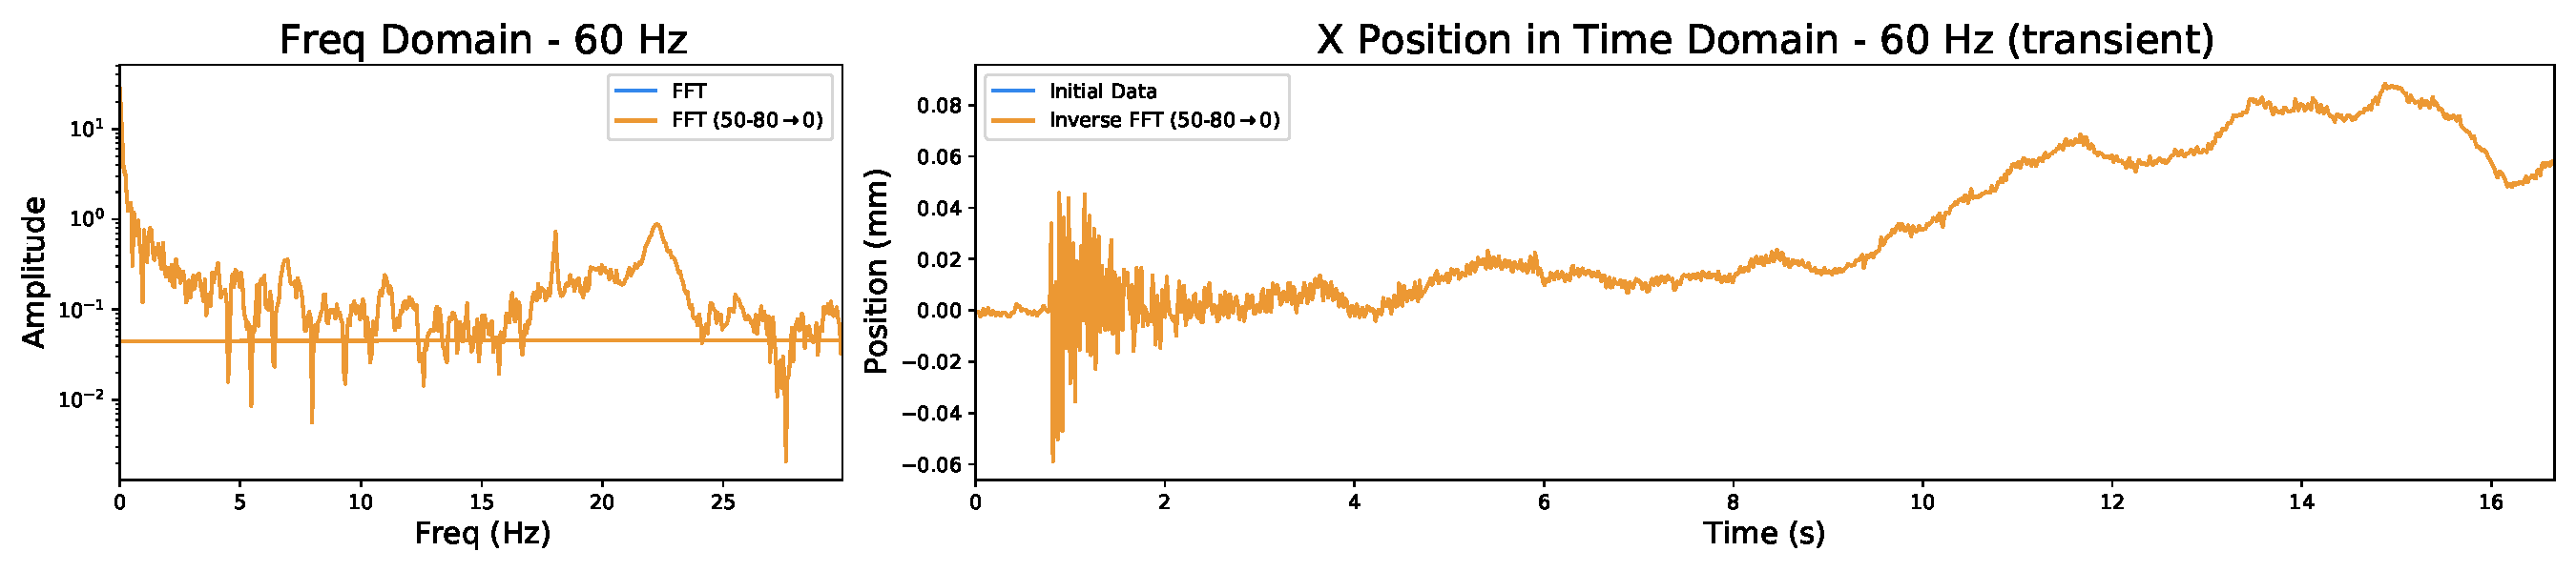
\includegraphics[width=\textwidth]{data_02_x_pos.pdf}
    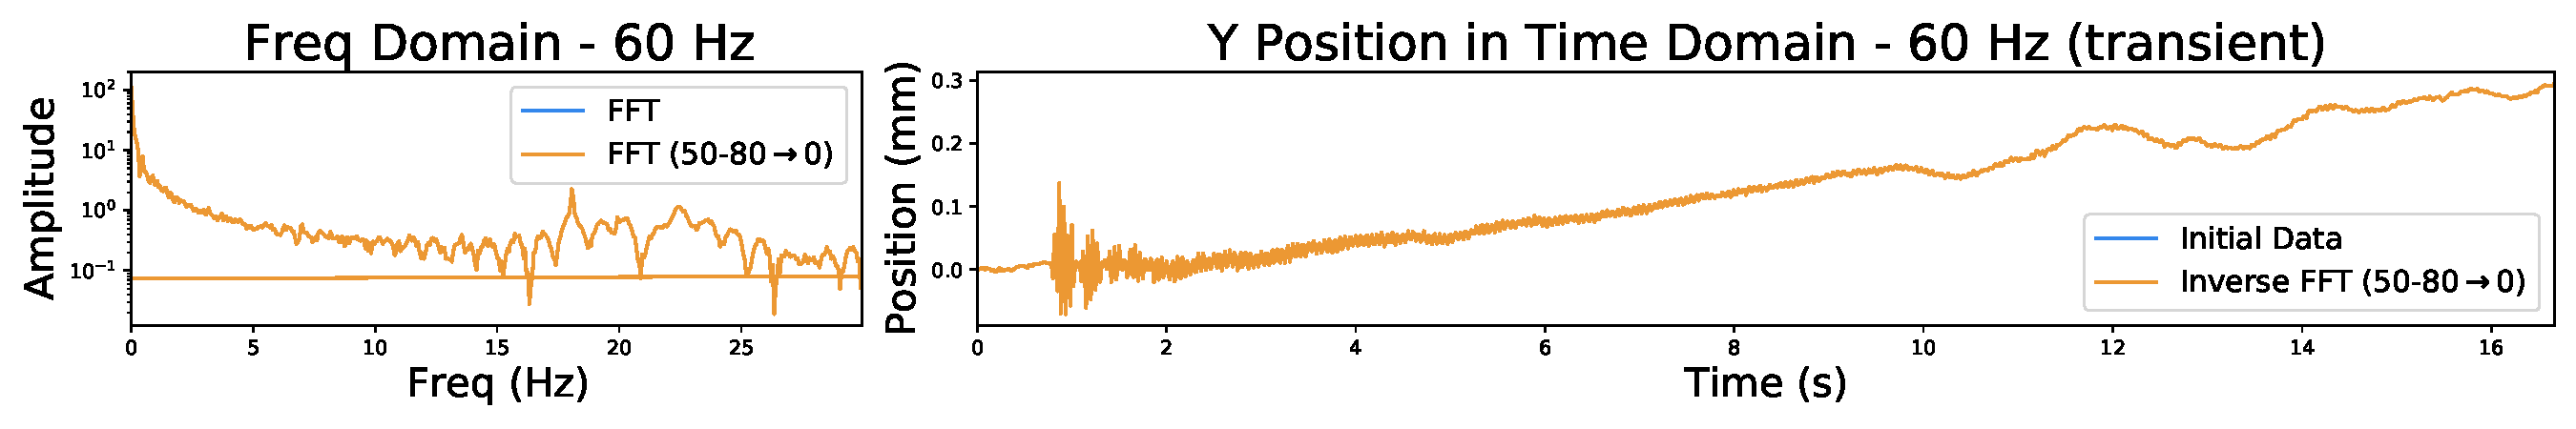
\includegraphics[width=\textwidth]{data_02_y_pos.pdf}
    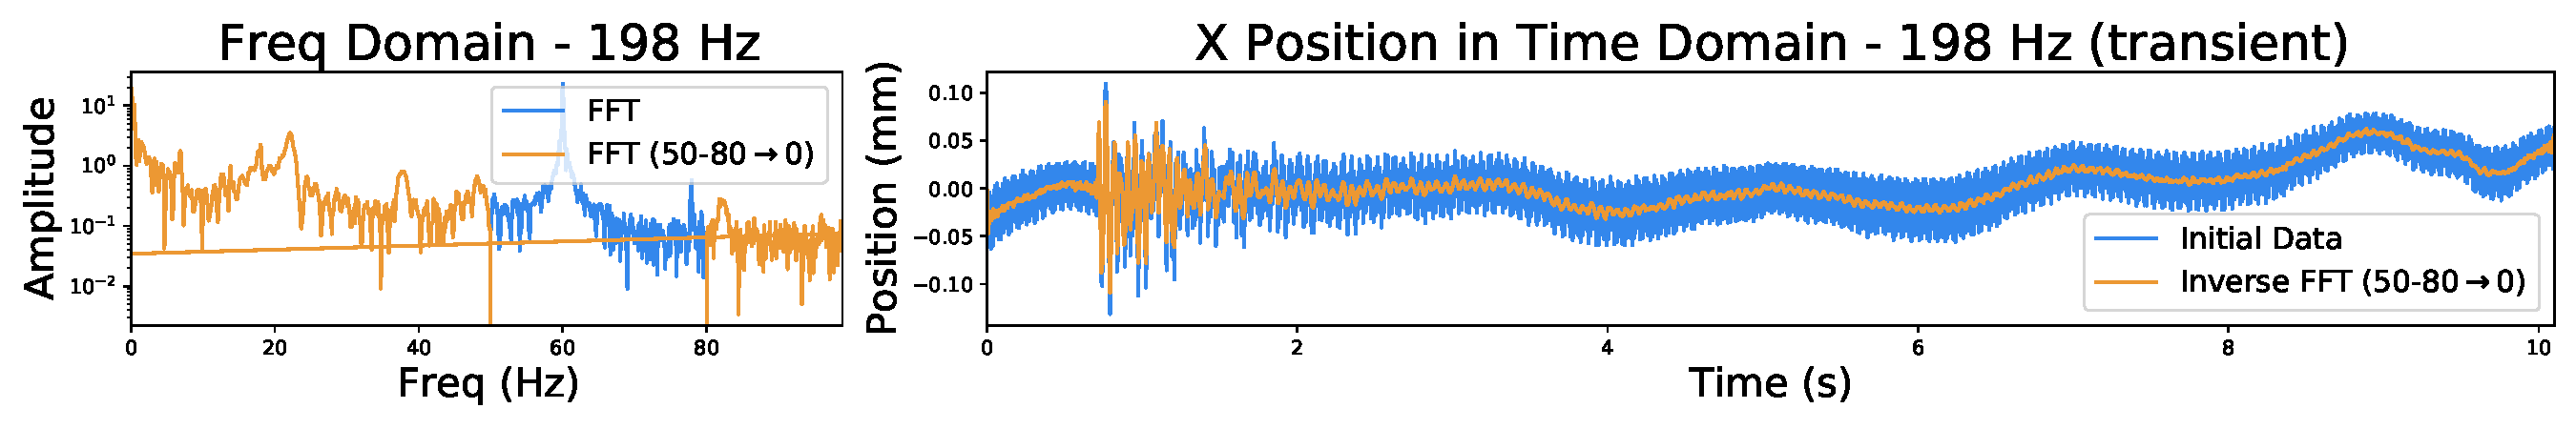
\includegraphics[width=\textwidth]{data_05_x_pos.pdf}
    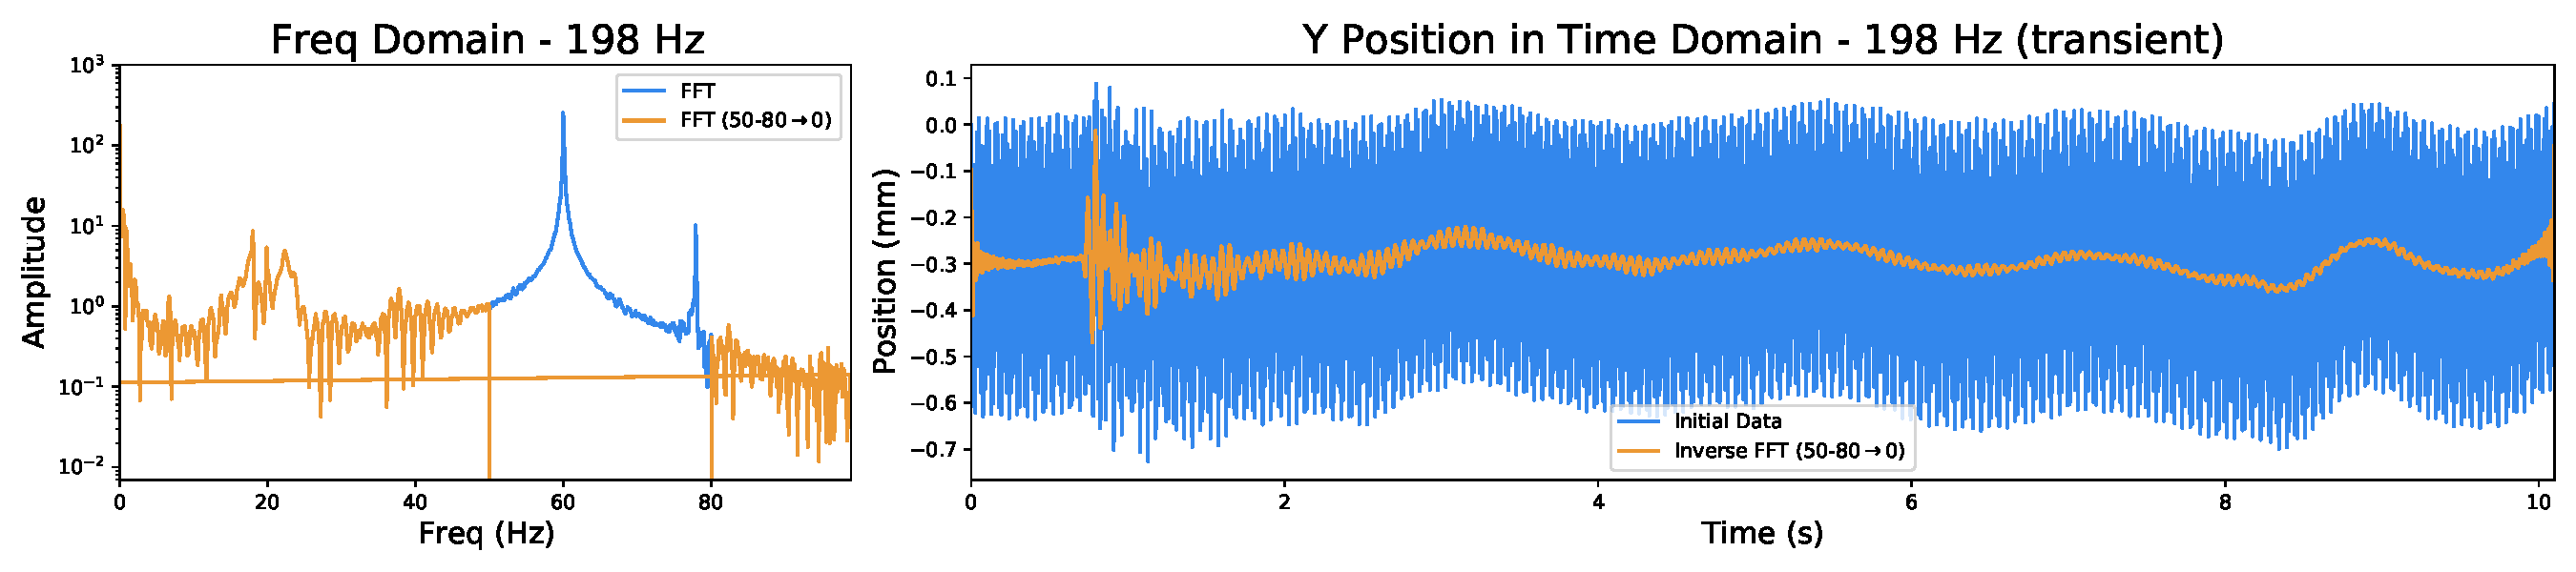
\includegraphics[width=\textwidth]{data_05_y_pos.pdf}
	\caption{The position data for the introduction of an outside impulse to study the transient behavior. Again, the effects of the FFT analysis can be seen in the 198 Hz capture.}
    \label{fig:trans_pos}
\end{figure}

\begin{figure}[!ht]
\centering\
    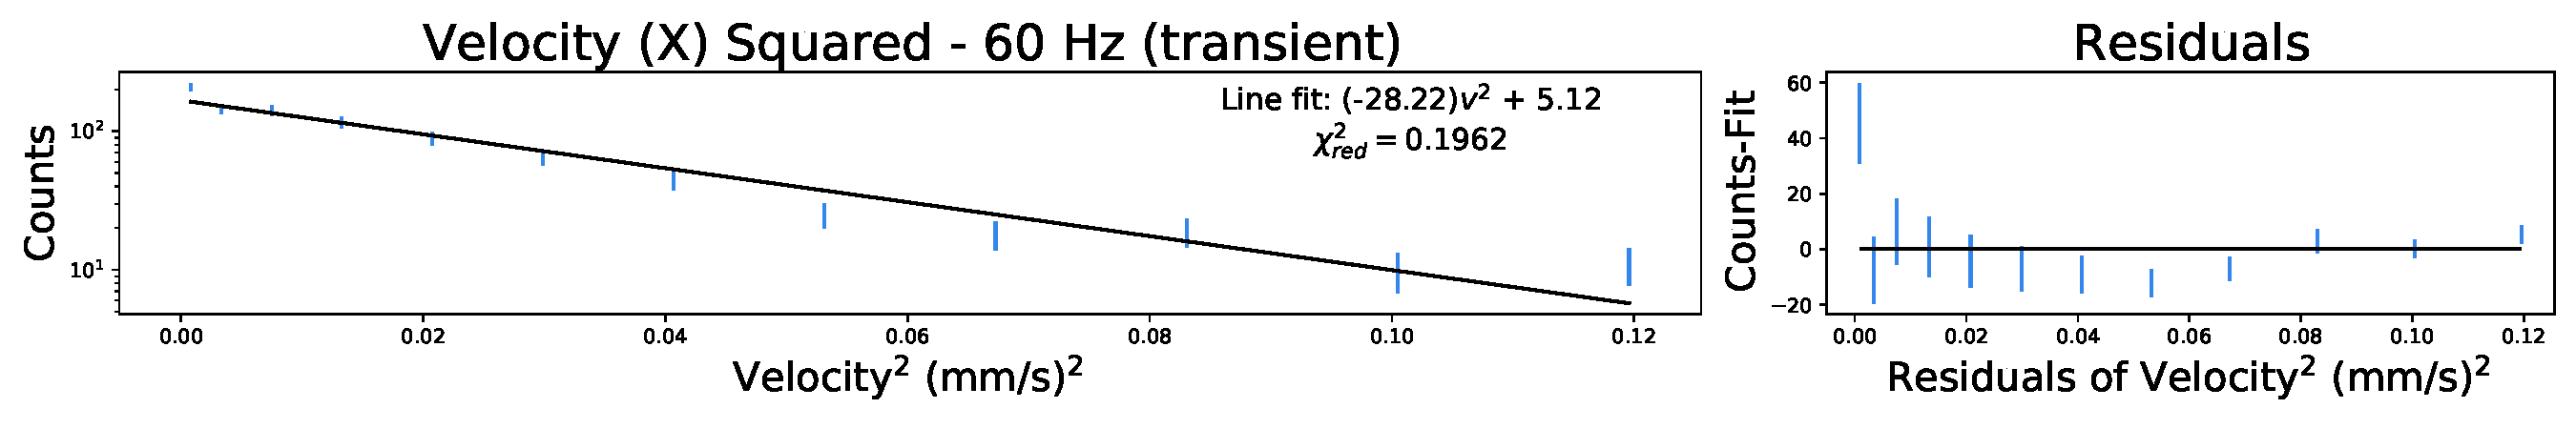
\includegraphics[width=\textwidth]{data_02_x_vel.pdf}
    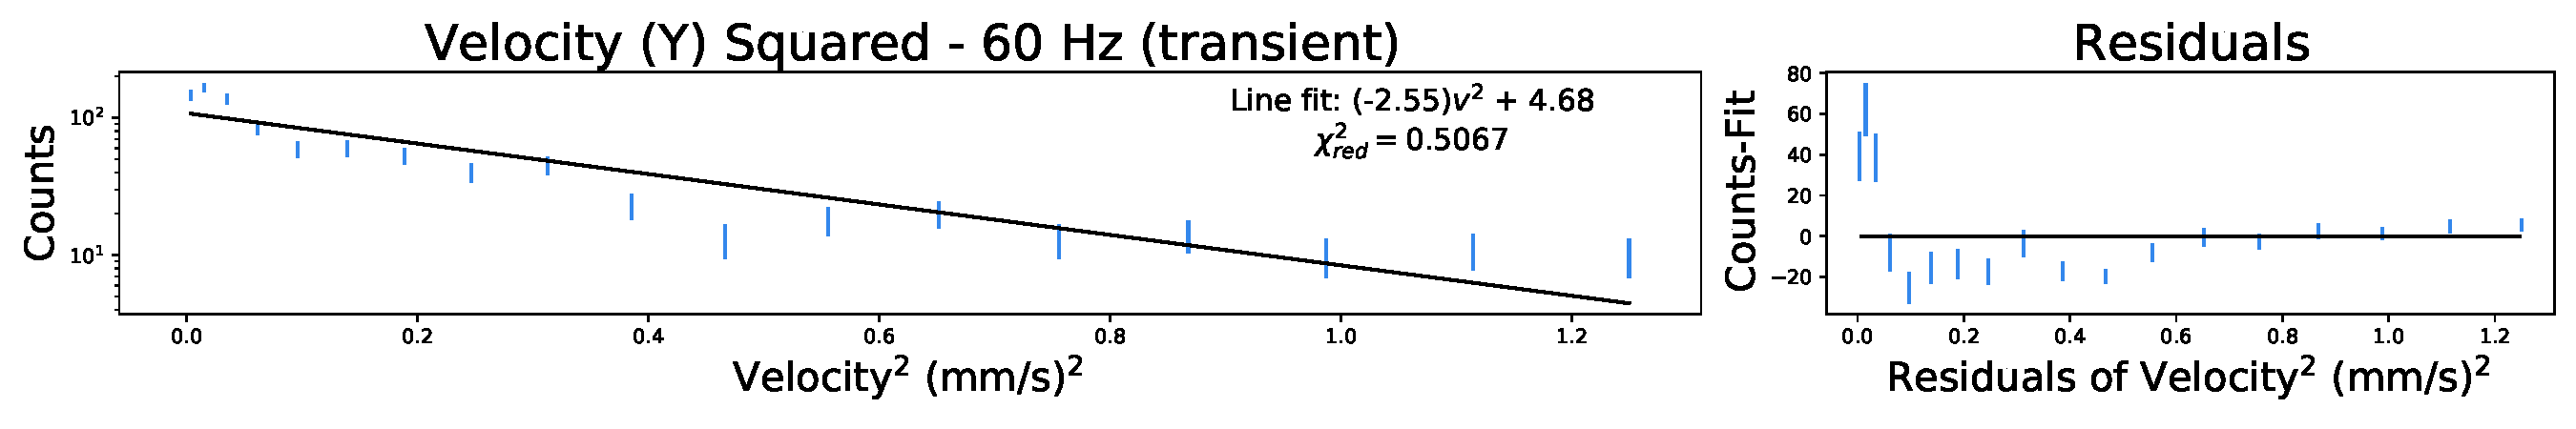
\includegraphics[width=\textwidth]{data_02_y_vel.pdf}
    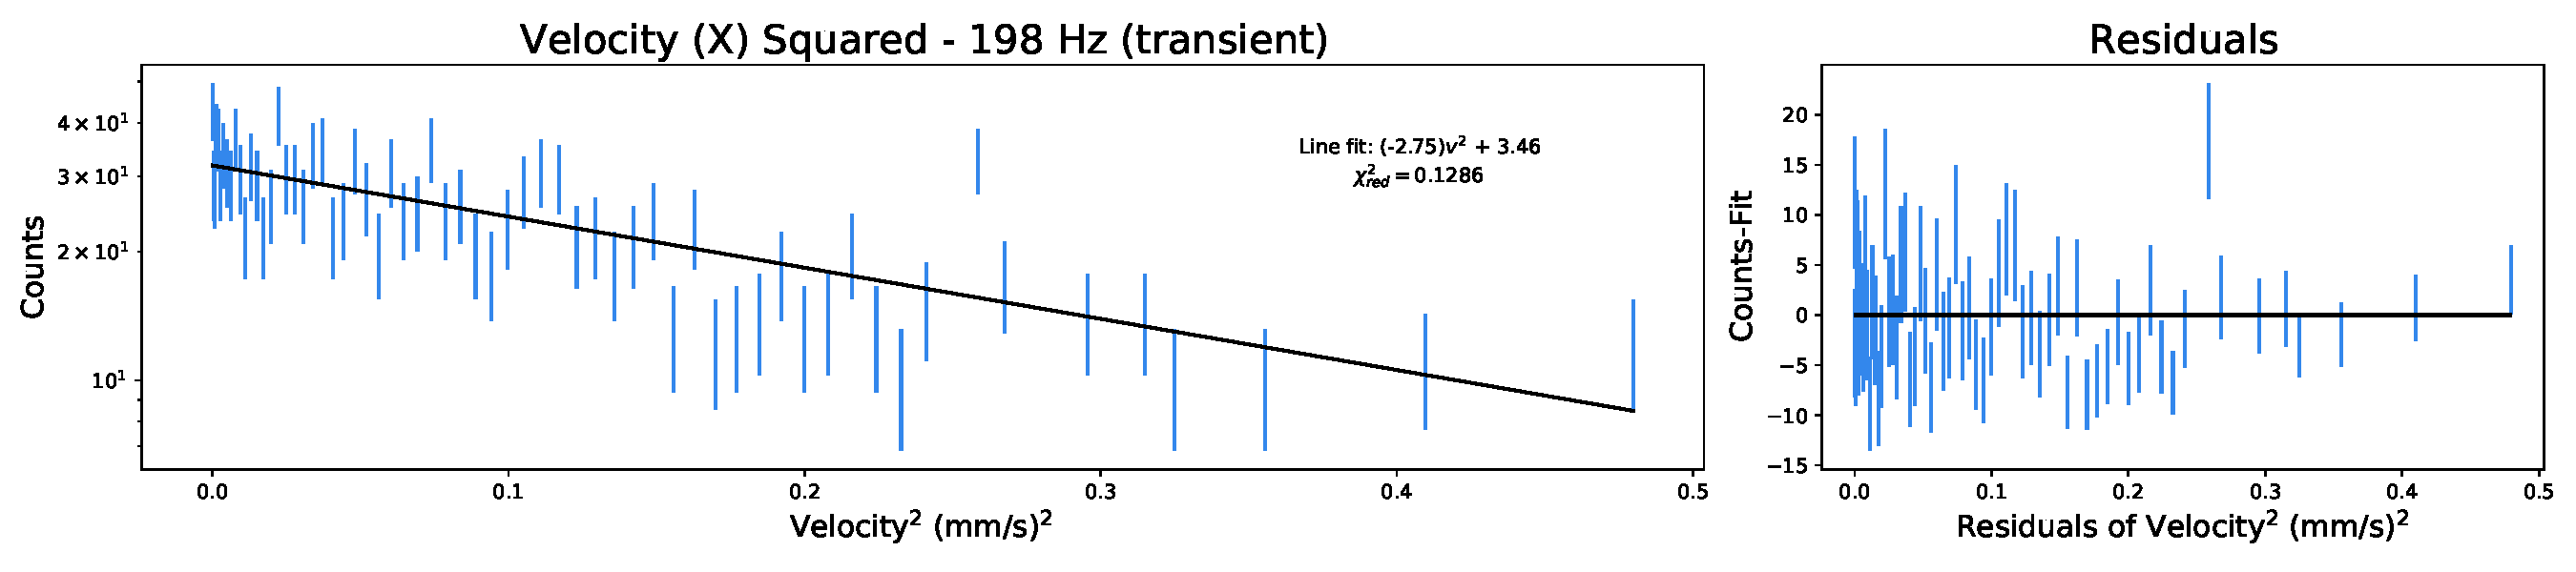
\includegraphics[width=\textwidth]{data_05_x_vel.pdf}
    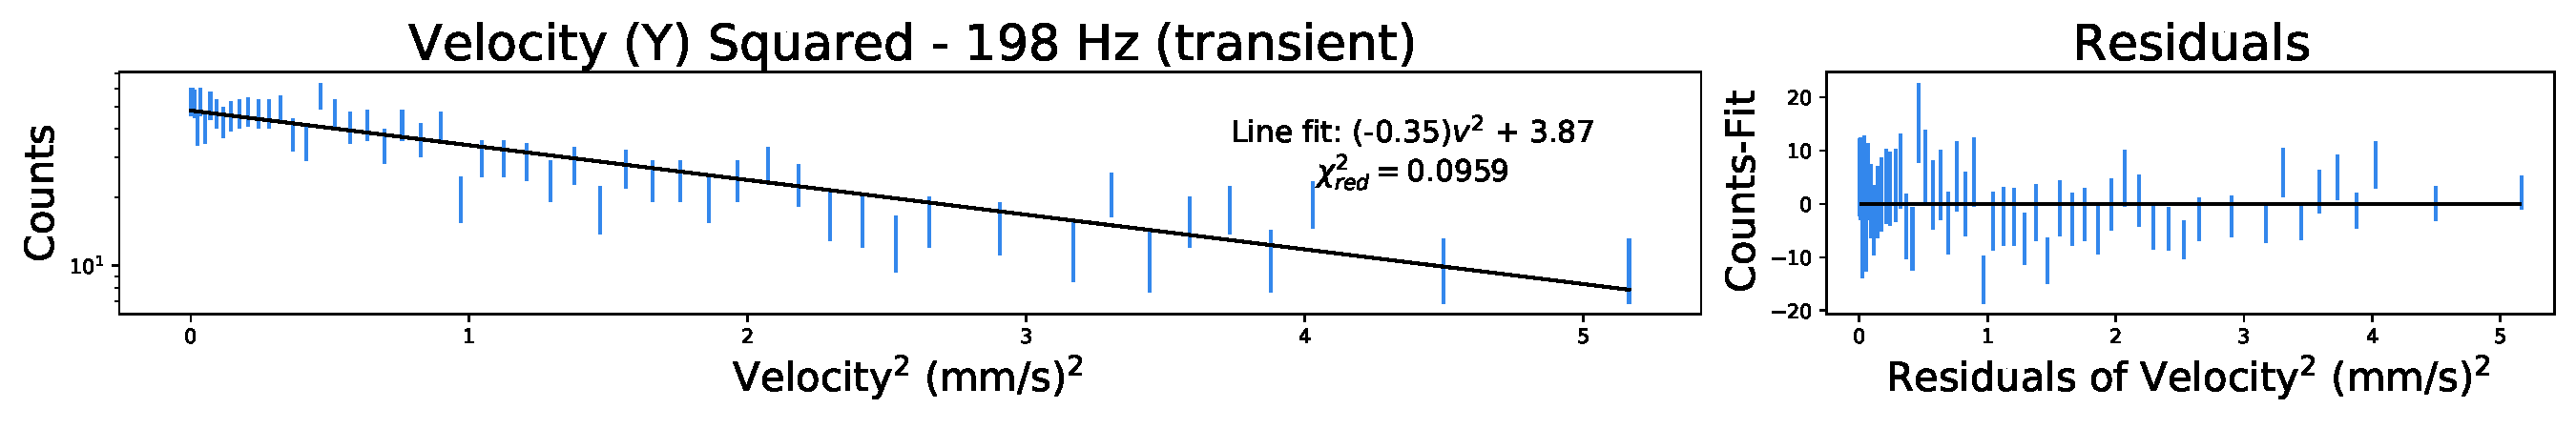
\includegraphics[width=\textwidth]{data_05_y_vel.pdf}
	\caption{The velocity histograms of both of the transient fits. The 60 Hz fit seems to be a little weaker according to the residuals, but the 198 Hz fit looks very good according to the residuals.}
    \label{fig:trans_vel}
\end{figure}

Another point of study in this lab was the transient response of the particle to a suddenly impulse of force on the surrounding environment. To simulate this, the table near the trap was bumped with the back of the hand. The resulting impact to the position and velocity can be seen in Figure \ref{fig:trans_pos}. Looking at the Fourier analysis, the same exact strategy seems to work well here as well. It can be seen, especially in the velocity data, that the bump introduced some more kinetic energy and made a linear fit less ideal, more for the 60 Hz trial than the 198 Hz trial. 

\begin{table}[ht]
\caption{}
\label{tab:trans_masses}
\centering
\begin{tabular}{lllll}
Freq   & Axis & Num of Bins & Mass (pg)     & $\chi_\text{red}^2$ \\ \hline
60 Hz  & X    & 200         & $232 \pm  17$ & 0.196               \\
       & Y    & 200         & $21 \pm 2$    & 0.507               \\
198 Hz & X    & 2000        & $23 \pm 2$    & 0.129               \\
       & Y    & 1000        & $2.9 \pm 0.2$ & 0.096              
\end{tabular}
\end{table}

Comparing the masses with those given in the absence of such an impulse, a large discrepency can be seen. Primarily, the masses observed are much smaller. We know, however, that this is the same particle that we got the masses in Table \ref{tab:masses}, so there must be another explanation than a sudden change in mass. This is a result of the particles having extra kinetic energy from the impulse that is attributed to thermal energy in the math. Consequently, the mass must be lighter to move faster with the same amount of ambient energy. This is an important conclusion to draw from about particle traps in general: outside impulses are important to consider. 

\subsection{Coulomb Crystal}
%% Give the pics of crystal and analysis that a recording gave. 
\begin{figure}[!ht]
\centering
    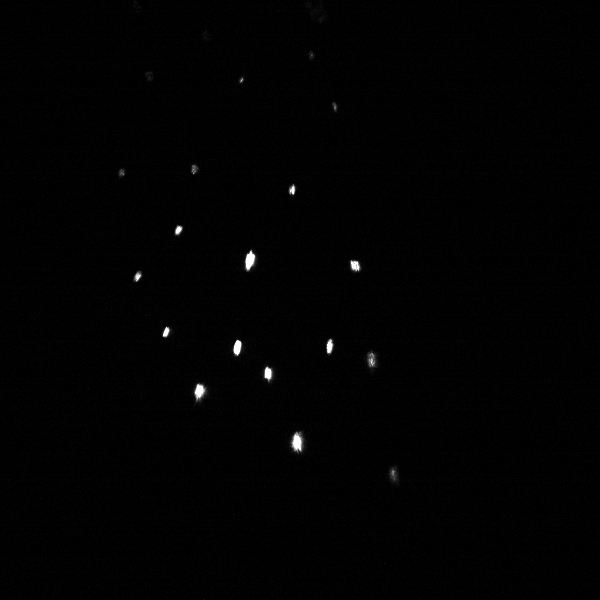
\includegraphics[width=0.45\textwidth]{crystal_1.PNG}
    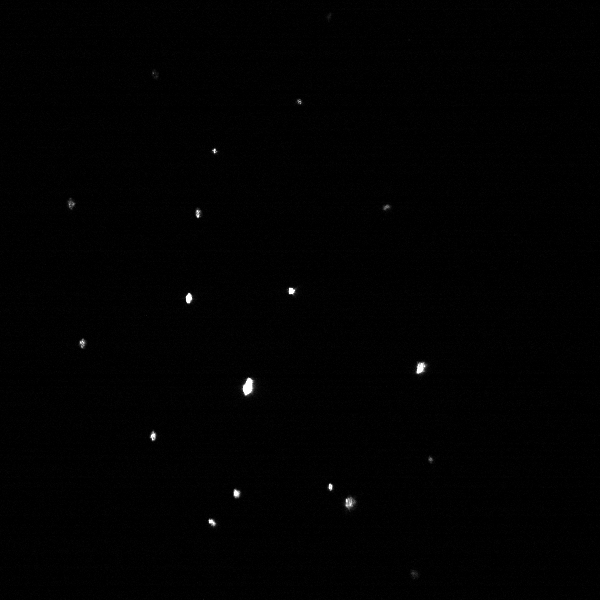
\includegraphics[width=0.45\textwidth]{crystal_2.PNG}
	\caption{Two captures of the same Coulomb Crystal.}
    \label{fig:crystals}
\end{figure}

When multiple charged particles are loaded into a trap at the same time they form a pseudo-stable arrangement. This arrangement looks similar to a crystal structure and can be seen to exist in all three dimensions; the properties are a lot easier to see when recorded. This structure is the result of the repulsive coulomb force that charged particles exert on each other; thus, a fitting name for this is a Coulomb Crystal. While the characteristics of micro-motion and secular motion are both present in this crystal and the analysis of the electric interaction between the particles may provide a more robust calculation of the mass, the code provided doesn't handle multiple particles well. So, this is a cool structure and a potentially useful one, but ultimately it had to be disrupted on numerous cases so that only one particle remained and the analysis could actually be done. 


%-----------------------------------------------------------------------

\section{Discussion and Conclusions}

This lab provided many learning experiments, both about personal shortcomings in experimental methods and also in the importance of certain environmental factors. Due diligence needs to be taken to understand the effects of important characteristics of the data being observed. When something does seem to be off, it's the responsibility of the experimenter to understand it and fix the error. It also was highlighted, through the \textbf{Transient Response} that watching out for unexpected sources of noise is importance. In a Colloquium given by Brian D'Urso for the MSU physics faculty, he pointed out that care has to be taken to not run important trials during common class times, as the rhythmic walking outside of the lab is enough to mess up the measurements. It's been shown that when that source is extremely predictable, such as with a 60 Hz AC source, that it can effectively be removed in the Fourier domain. However, when there is no clear peak, removing the data is not trivial, and possibly improbable without a deep dive into all of the sources of the noise. 

On top of the important lessons learned, an approximation of the mass of a particle was achieved; giving about $24.8 \pm 0.3$ pg. The physics that also gave the measurement of $925 \pm 63$ pg is not fully understood, but a convincing reason that the former is more trustworthy had been given. Beyond the mass, a good characteristic of the EIT could be seen, as the coulomb crystal. Theoretically this coulomb crystal could be used to give another measurement of the charge on each of the particles in the trap, giving way to calculating the force and another way of relating mass and displacement.


%-----------------------------------------------------------------------
\newpage
\clearpage
\section*{Appendix A}


\begin{longtable}{lllll}
\caption{The collected data from running many different bin sizes on the data. The following are the relation of the ``data\_num": 1 - 60 Hz, 2 - 60 Hz (transient), 3 - 61 Hz, 4 - 198 Hz, 5 - 198 Hz (transient), 33 - 60 Hz (bad), 36 - 200 Hz (bad)}
\label{tab:calc_data}\\
data\_num & variable & bins & calculated\_mass             & chi\textasciicircum{}2 \\
1         & y        & 35   & 523.28514 pg +/- 46.49112 pg & 0.726                  \\
1         & x        & 35   & 924.69180 pg +/- 62.82066 pg & 0.457                  \\
2         & y        & 75   & 17.24134 pg +/- 3.10498 pg   & 0.844                  \\
2         & y        & 100  & 18.00108 pg +/- 2.44132 pg   & 0.664                  \\
2         & y        & 200  & 21.00448 pg +/- 2.34851 pg   & 0.507                  \\
2         & x        & 200  & 232.31192 pg +/- 17.36094 pg & 0.196                  \\
3         & y        & 50   & -0.66282 pg +/- 0.20780 pg   & 0.555                  \\
3         & y        & 100  & -0.99388 pg +/- 0.11654 pg   & 0.218                  \\
3         & y        & 200  & -0.80153 pg +/- 0.11592 pg   & 0.240                  \\
3         & x        & 50   & 132.04445 pg +/- 12.89677 pg & 0.594                  \\
3         & x        & 100  & 131.56066 pg +/- 6.47084 pg  & 0.171                  \\
3         & x        & 200  & 132.63179 pg +/- 6.51265 pg  & 0.170                  \\
4         & y        & 200  & 20.45896 pg +/- 0.42721 pg   & 0.086                  \\
4         & y        & 500  & 22.23804 pg +/- 0.55817 pg   & 0.159                  \\
4         & y        & 1000 & 23.55828 pg +/- 0.40332 pg   & 0.096                  \\
4         & y        & 2000 & 24.37536 pg +/- 0.34902 pg   & 0.078                  \\
4         & y        & 5000 & 24.87292 pg +/- 0.35429 pg   & 0.075                  \\
4         & x        & 200  & 52.06898 pg +/- 0.57280 pg   & 0.039                  \\
4         & x        & 500  & 52.64460 pg +/- 0.70130 pg   & 0.067                  \\
4         & x        & 1000 & 52.86629 pg +/- 0.72387 pg   & 0.074                  \\
4         & x        & 2000 & 51.32041 pg +/- 0.82213 pg   & 0.081                  \\
4         & x        & 5000 & 46.72509 pg +/- 1.18683 pg   & 0.090                  \\
5         & x        & 200  & 11.63175 pg +/- 1.36204 pg   & 1.094                  \\
5         & x        & 500  & 24.83700 pg +/- 1.03062 pg   & 0.080                  \\
5         & x        & 1000 & 25.71883 pg +/- 1.29461 pg   & 0.096                  \\
5         & x        & 2000 & 22.67917 pg +/- 2.35722 pg   & 0.129                  \\
5         & x        & 5000 & 3.03607 pg +/- 3.38284 pg    & 0.077                  \\
5         & y        & 200  & 1.72155 pg +/- 0.20595 pg    & 0.836                  \\
5         & y        & 500  & 2.90765 pg +/- 0.12980 pg    & 0.086                  \\
5         & y        & 1000 & 2.88800 pg +/- 0.17400 pg    & 0.096                  \\
5         & y        & 2000 & 2.21042 pg +/- 0.24083 pg    & 0.102                  \\
5         & y        & 5000 & 0.35675 pg +/- 0.51552 pg    & 0.043                  \\
33        & x        & 20   & 0.22677 pg +/- 0.02863 pg    & 0.661                  \\
33        & x        & 50   & 0.31130 pg +/- 0.03220 pg    & 0.363                  \\
33        & x        & 100  & 0.39298 pg +/- 0.03882 pg    & 0.233                  \\
33        & x        & 200  & 0.42264 pg +/- 0.05401 pg    & 0.174                  \\
33        & x        & 200  & 0.42264 pg +/- 0.05401 pg    & 0.174                  \\
33        & y        & 100  & 0.39298 pg +/- 0.03882 pg    & 0.233                  \\
33        & y        & 200  & 0.47200 pg +/- 0.05171 pg    & 0.457                  \\
33        & y        & 500  & 0.56779 pg +/- 0.06627 pg    & 0.378                  \\
33        & y        & 1000 & 0.81340 pg +/- 0.09257 pg    & 0.222                  \\
33        & y        & 2000 & 0.75544 pg +/- 0.10195 pg    & 0.199                  \\
36        & x        & 20   & 0.03328 pg +/- 0.00313 pg    & 0.297                  \\
36        & x        & 30   & 0.03569 pg +/- 0.00305 pg    & 0.256                  \\
36        & x        & 50   & 0.04038 pg +/- 0.00340 pg    & 0.221                  \\
36        & x        & 100  & 0.04256 pg +/- 0.00437 pg    & 0.227                  \\
36        & x        & 200  & 0.05403 pg +/- 0.00756 pg    & 0.122                  \\
36        & y        & 100  & 0.01772 pg +/- 0.00269 pg    & 1.032                  \\
36        & y        & 200  & 0.02565 pg +/- 0.00303 pg    & 0.568                  \\
36        & y        & 500  & 0.03717 pg +/- 0.00370 pg    & 0.236                  \\
36        & y        & 1000 & 0.04501 pg +/- 0.00577 pg    & 0.187                  \\
36        & y        & 2000 & 0.03722 pg +/- 0.00744 pg    & 0.139                  \\
\end{longtable}


%-----------------------------------------------------------------------




\vskip 0.2in
\bibliography{lab04}


\end{document}
